\documentclass{article}

\usepackage{float} % Float control

\usepackage{listings} % Code listings
\usepackage{lstautogobble} % Fix relative indenting
\usepackage{xcolor} % Code coloring
\usepackage{zi4} % Nice font

\definecolor{bluekeywords}{rgb}{0.13, 0.13, 1}
\definecolor{greencomments}{rgb}{0, 0.5, 0}
\definecolor{redstrings}{RGB}{163, 21, 21}
\definecolor{graynumbers}{rgb}{0.5, 0.5, 0.5}

\lstset{
    autogobble,
    columns=fullflexible,
    numbers=left,
    showspaces=false,
    showtabs=false,
    breaklines=true,
    showstringspaces=false,
    breakatwhitespace=true,
    escapeinside={(*@}{@*)},
    commentstyle=\color{greencomments},
    keywordstyle=\color{bluekeywords},
    stringstyle=\color{redstrings},
    numberstyle=\color{graynumbers},
    basicstyle=\ttfamily\footnotesize,
    xleftmargin=2em,
    tabsize=4,
    captionpos=b
}


\usepackage{geometry}
\usepackage{amsmath}
\usepackage[utf8]{inputenc}
\usepackage{amssymb}
\usepackage{amsxtra}
\usepackage{listings}
\usepackage{graphicx}
\usepackage[labelfont=bf]{caption}
\usepackage{subcaption}
\usepackage{cite}
\usepackage[hidelinks]{hyperref}
\usepackage{todonotes}
\usepackage{booktabs}
\usepackage{nicematrix}

\graphicspath{{../figures/}}

\newcommand{\titleVariableHead}{}
\newcommand{\titleVariableMain}{}
\newcommand{\titleVariableSub}{}

\newcommand{\titlehead}[1]{\renewcommand{\titleVariableHead}{#1}}
\newcommand{\titlemain}[1]{\renewcommand{\titleVariableMain}{#1}}
\newcommand{\titlesub}[1]{\renewcommand{\titleVariableSub}{#1}}

\newcommand{\maketitleandtoc}{
  \maketitle
  \thispagestyle{empty}
  \newpage

  \tableofcontents
  \thispagestyle{empty}
  \newpage

  \pagestyle{headings}
  \setcounter{page}{1}
}

\newcommand{\makebibliography}{
  \newpage
  \nocite{}
  \bibliographystyle{plain}
  \bibliography{references}
}

\title{
{\bf \scriptsize \titleVariableHead} \\[3cm]
{\Huge \titleVariableMain} \\
{\large \titleVariableSub} \\[2cm]
}



\titlehead{
  RHEINISCH-WESTF\"ALISCHE TECHNISCHE HOCHSCHULE AACHEN\\
  Laboratory Course Astronomy and Astrophysics
}
\titlemain{Stellar Statistics}
\titlesub{Seminar Report}
\author{Marco Bischoff (Matr. No. 370222)}

\begin{document}

\maketitleandtoc

\section{Introduction}
\label{sec:introduction}

Identifying stars in astronomical images and estimating their brightness are fundamental
tasks in astronomy and commonly the first steps in many astronomical analyses. Night sky
images are often contaminated by other sources of light and contain biases that must be
corrected before the images can be analyzed. In this paper, I present approaches to
correct for various sources of bias in astronomical images, identify stars in the images,
estimate their magnitudes and use these magnitudes to do further analysis. The final goal
is to estimate the source-count distribution of stars in the images and compare it to the
literature.

\subsection{Software Library}
\label{sec:software-library}

The methods presented in this paper are implemented in a software library called
\texttt{brightest}. It is designed with a focus on reusability and extensibility, such
that the methods are not optimized for the specific images used in this paper, but can be
applied to any set of astronomical images. The code is written in Python 3.12 and is
available \href{https://github.com/bischoff-m/brightest}{on GitHub} \cite{Bischoff2025}.
The most important libraries used, their versions and their purpose are listed in
\autoref{tab:libraries}. This list represents the current state and may change in the
future.

\begin{table}[htbp]
  \centering
  \begin{tabular}{lll}
    \toprule
    Library                                   & Version   & Purpose                                 \\
    \midrule
    \texttt{astrometry} \cite{astrometry2010} & 4.1.2     & Solving for position                    \\
    \texttt{astropy} \cite{astropy2022}       & 7.0.1     & Pixel-to-sky mapping                    \\
    \texttt{astroquery} \cite{astroquery2019} & 0.4.9     & Querying the SIMBAD database            \\
    \texttt{opencv-python} \cite{opencv2000}  & 4.11.0.86 & Image processing                        \\
    \texttt{rawkit} \cite{rawkit2025}         & 0.6.0     & Reading raw images (wrapper for LibRaw) \\
    \texttt{scikit-learn} \cite{scikit-learn} & 1.6.1     & K-means clustering                      \\
    \bottomrule
  \end{tabular}
  \caption{Most notable dependencies of the \texttt{brightest} library.}
  \label{tab:libraries}
\end{table}


\section{Image Calibration}
\label{sec:image-calibration}

The first step in the analysis is to preprocess the raw images to correct for various
sources of noise. This is necessary for the star identification, magnitude estimation and
other analyses the user might want to perform to give accurate results. In this section,
all steps of the preprocessing pipeline are described in detail. First, the observations
that I used for testing are described in \autoref{sec:observations}. Reading the raw image
data is covered in \autoref{sec:raw-image-data}. The subsequent processing steps are pixel
correction (\autoref{sec:faulty-pixels}), vignetting correction
(\autoref{sec:vignetting-correction}), interpolation (\autoref{sec:interpolation}) and
skyglow correction (\autoref{sec:skyglow-correction}). Finally, the full pipeline with
some minor additional processing steps is described in \autoref{sec:full-pipeline}.

\subsection{Observations}
\label{sec:observations}

To test my processing pipeline and perform the analysis, I used a set of wide-field images
photographed with a Canon EOS 1200D camera and a 18-55 mm lens, mounted on a tripod. The
images were taken in the Stadtpark in Aachen and under good weather conditions. Even
though images taken under perfect conditions would be ideal for estimating the
source-count distribution, they would not be ideal for testing the robustness of the
methods. The pipeline is able to handle different types of noise and bias, like faulty
pixels (\autoref{sec:faulty-pixels}) and skyglow (\autoref{sec:skyglow-correction}). I
selected the best image and used it for the analysis to keep the results comparable. The
camera settings for this image are shown in \autoref{tab:camera-settings}. In general, I
varied the exposure time and ISO settings to capture images with different levels of
brightness and noise. All images were taken with an aperture of f/3.5 and a focal length
of 18 mm and were saved in the Canon CR2 raw image format. An example image is shown in
\autoref{fig:sky-input}.

\begin{table}[b]
  \centering
  \begin{tabular}{ll}
    \toprule
    \textbf{Parameter} & \textbf{Value}        \\
    \midrule
    Sensor size        & $22.3 \times 14.9$ mm \\
    Image resolution   & $5202 \times 3465$ px \\
    Bit depth          & 14 bits               \\
    Aperture           & f/3.5                 \\
    Focal length       & 18 mm                 \\
    Exposure time      & 10 s                  \\
    ISO                & 6400                  \\
    \bottomrule
  \end{tabular}
  \caption{Camera specifications and settings for the night sky image used throughout this paper.}
  \label{tab:camera-settings}
\end{table}

\begin{figure}[tb]
  \centering
  \begin{subfigure}{.45\textwidth}
    \centering
    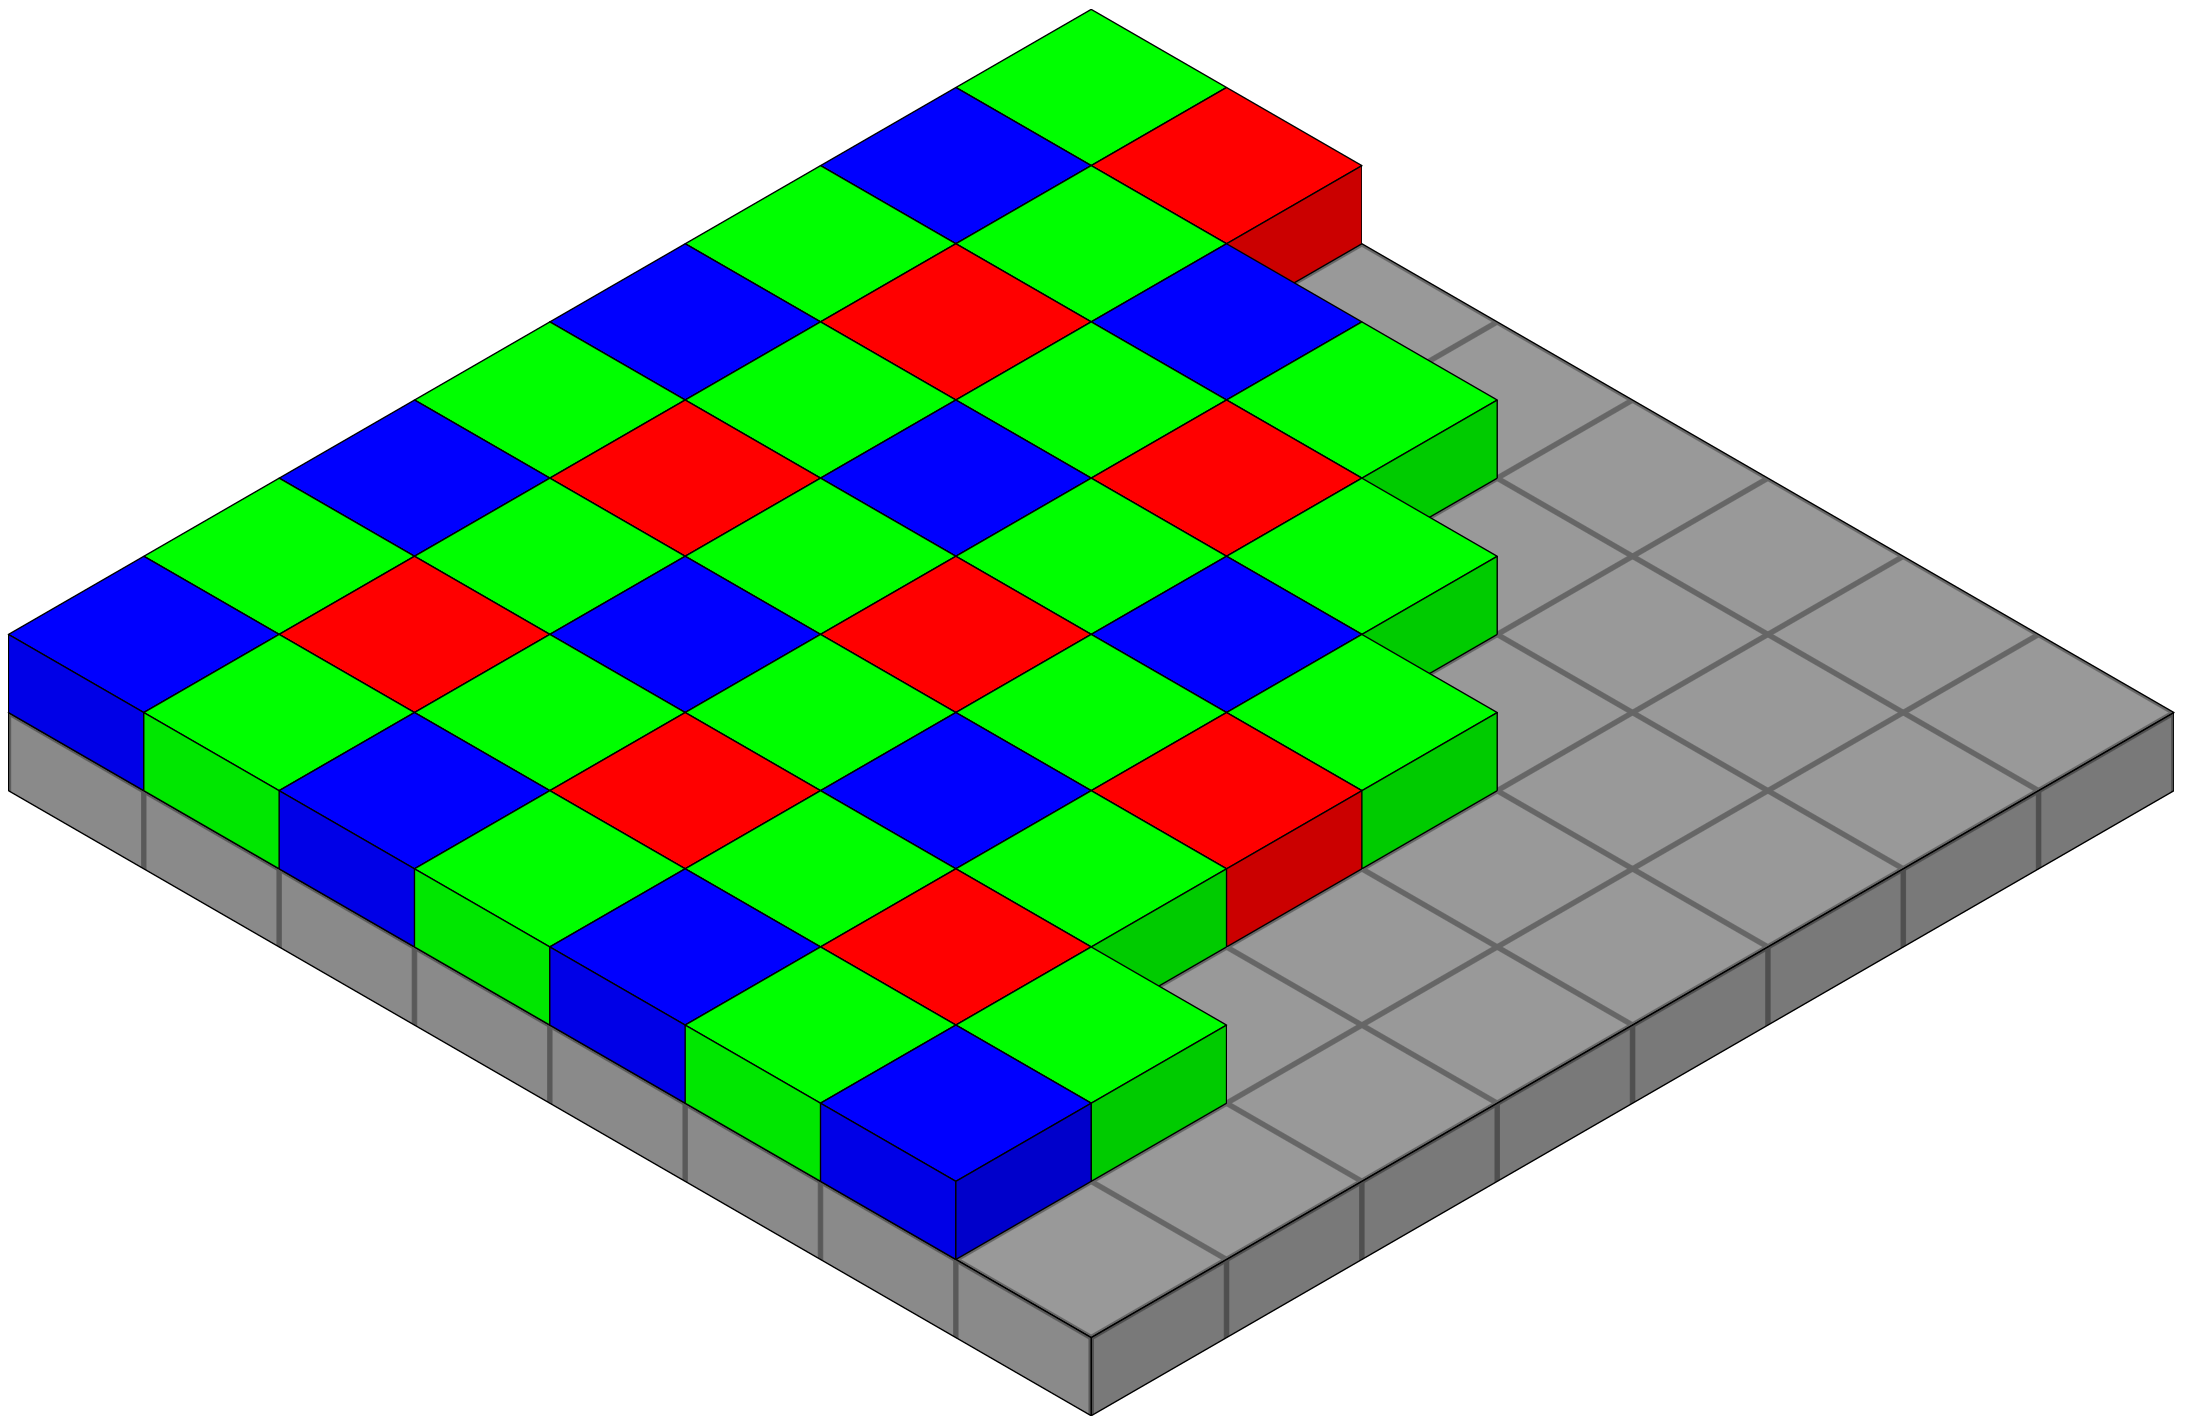
\includegraphics[width=.8\linewidth]{bayer-pattern.png}
    \caption{An example Bayer arrangement of color filters on the pixel array of an image sensor.}
    \label{fig:bayer-pattern}
  \end{subfigure}%
  \hfill
  \begin{subfigure}{.45\textwidth}
    \centering
    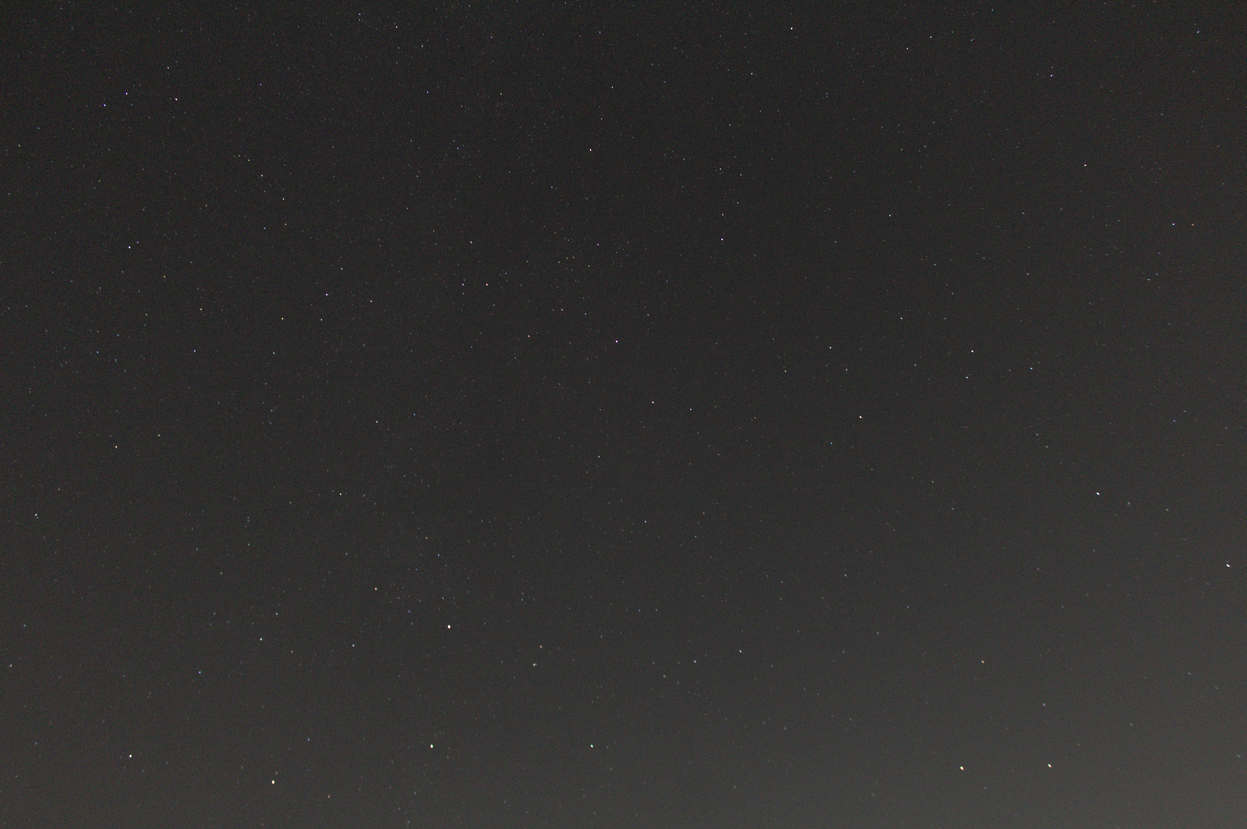
\includegraphics[width=\linewidth]{sky-input.png}
    \caption{The night sky image used throughout this paper, converted from raw to RGB.}
    \label{fig:sky-input}
  \end{subfigure}
  \caption{}
\end{figure}

In addition to the night sky images, I also took black and white field images for
calibration. The black images were taken with the lens cap on, before and after each set
of night sky images, to match the conditions of the night sky images as closely as
possible. The white images were taken out of focus, with a homogeneously illuminated white
paper covering the entire field of view. To avoid saturation of the sensor, the shutter
speed for the white images was set to 5 ms. The black images were used to reduce the noise
in dark pixels (\autoref{sec:full-pipeline}), while the white images were used to correct
for vignetting (\autoref{sec:vignetting-correction}).

\subsection{Raw Image Data}
\label{sec:raw-image-data}

Raw images store the unprocessed data captured by the camera sensor without any
modifications. For the Canon EOS 1200D, this is a matrix with values ranging from 0 to
16383, representing the intensity of light captured. Each pixel has a red, green or blue
color filter, corresponding to the Bayer pattern used by the camera. An example of a Bayer
arrangement is shown in \autoref{fig:bayer-pattern}. The camera that I used has the
following pattern:
\begin{align*}
  \begin{bmatrix}
    R & G \\
    G & B \\
  \end{bmatrix}
\end{align*}
This pattern is repeated for each $2 \times 2$ pixel block in the image. For my analysis,
I am only interested in the intensity of light, instead of the color. As 50\% of the
pixels in the image are green, I only use the green channel for further processing. All
methods of my software library can be used equally with the red and blue channels, but
this will not be discussed in this paper. I masked the red and blue pixels, which leaves a
checkerboard pattern of green pixels, as shown in \autoref{fig:faulty-pixels}. The missing
pixels will be filled in using interpolation (\autoref{sec:interpolation}), because the
methods from the OpenCV library require a complete image. However, it is important to
interpolate at the latest possible stage, to avoid introducing artifacts and additional
bias into the image. I used the \texttt{rawkit} library \cite{rawkit2025} to read the raw
images, which is a Python wrapper for the LibRaw library and also provides metadata about
the images.

I selected a night sky image with a high number of stars and a low level of noise to test
the processing pipeline and perform the analysis. The image was taken with an exposure
time of 10 s and an ISO setting of 6400 and is shown in \autoref{fig:sky-input}. In the
following sections, I will refer to this image with the red and blue channels masked as
the \textit{input image}.

\subsection{Faulty Pixels}
\label{sec:faulty-pixels}

\begin{figure}[tb]
  \centering
  \begin{subfigure}{.49\textwidth}
    \centering
    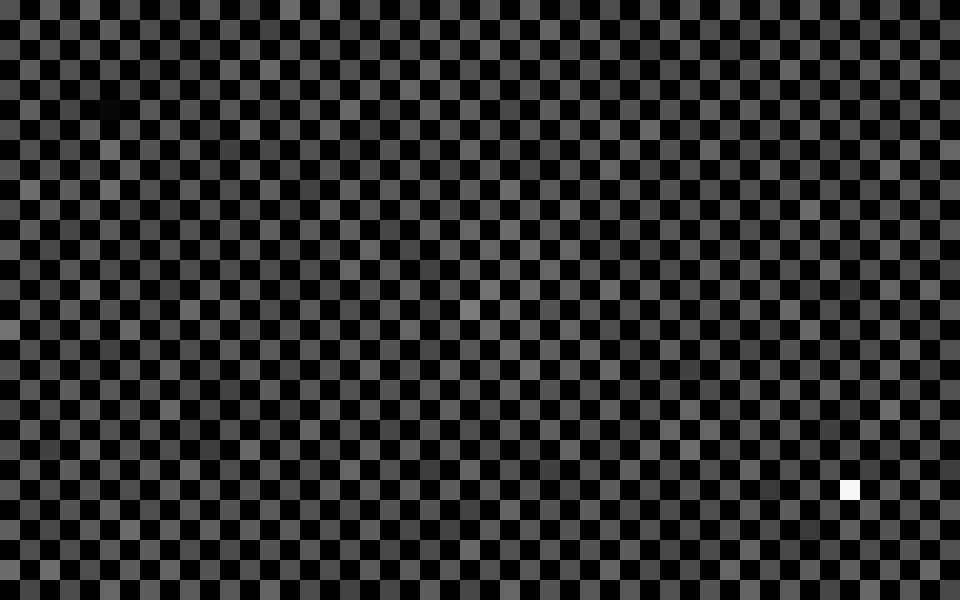
\includegraphics[width=\linewidth]{faulty-before.png}
    \caption{Before correction}
    \label{fig:faulty-before}
  \end{subfigure}%
  \hfill
  \begin{subfigure}{.49\textwidth}
    \centering
    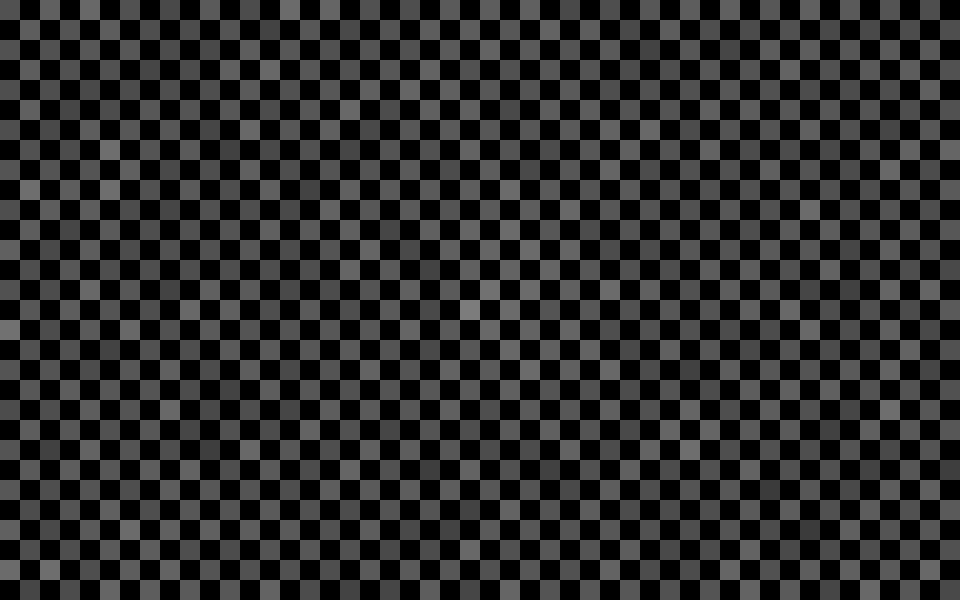
\includegraphics[width=\linewidth]{faulty-after.png}
    \caption{After correction}
    \label{fig:faulty-after}
  \end{subfigure}
  \caption{A cutout of the input image with a dead pixel in the top left and a hot pixel
    in the bottom right, before and after applying the method described in
    \autoref{sec:faulty-pixels}.}
  \label{fig:faulty-pixels}
\end{figure}

A pixel is considered faulty if it does not respond to light as expected. This needs to be
corrected before further analysis, as it can reduce the accuracy of finding stars or
predicting their magnitudes. I considered two types of faulty pixels. First, a pixel can
be permanently damaged due to a malfunction in the sensor, which can cause it to have an
incorrect sensitivity to light. Second, a pixel can be faulty due to cosmic rays or other
sources of radiation, which can cause it to receive more light than expected. Both types
result in a pixel that has a higher or lower intensity than its neighbors.

\begin{figure}[tbp]
  \centering
  \begin{subfigure}{.49\textwidth}
    \centering
    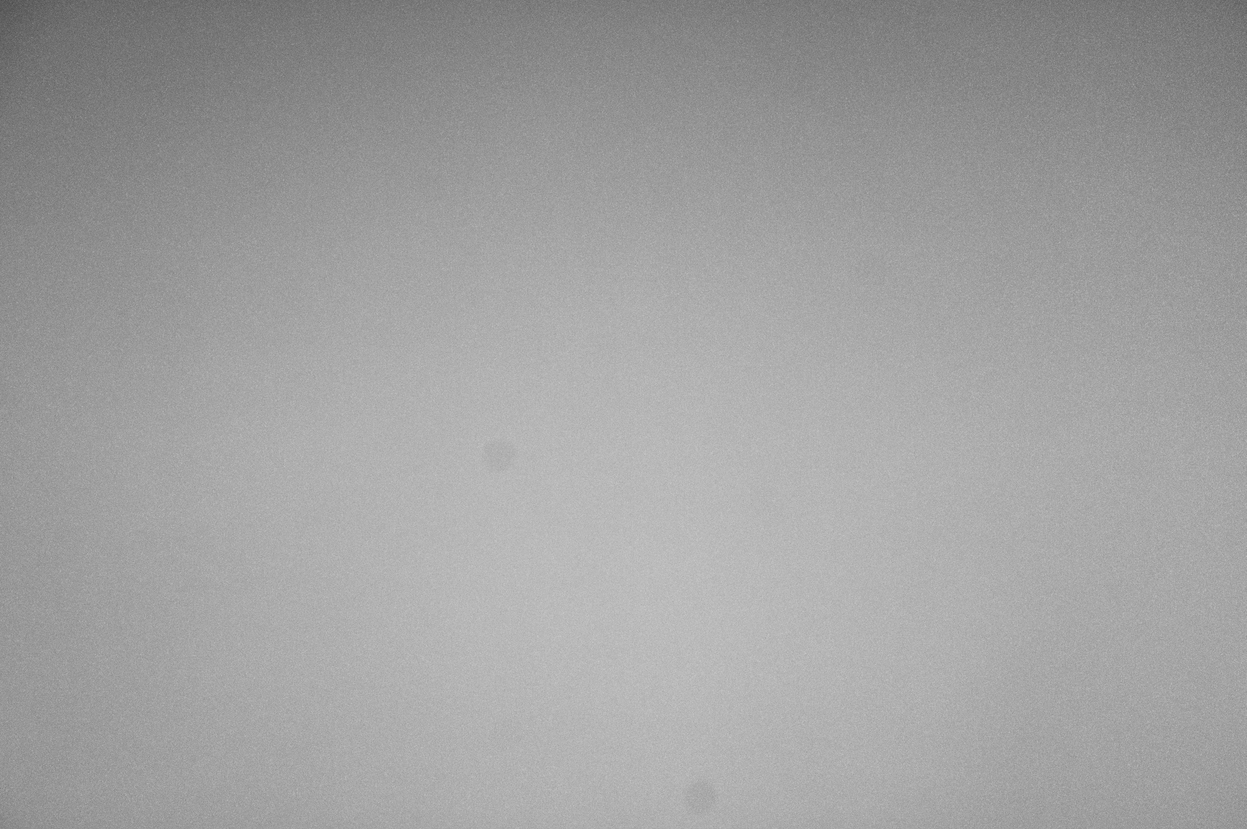
\includegraphics[width=\linewidth]{vignette-photo.png}
    \caption{The white field image with reduced brightness and increased contrast for better visualization.}
    \label{fig:vignette-photo}
  \end{subfigure}%
  \hfill
  \begin{subfigure}{.49\textwidth}
    \centering
    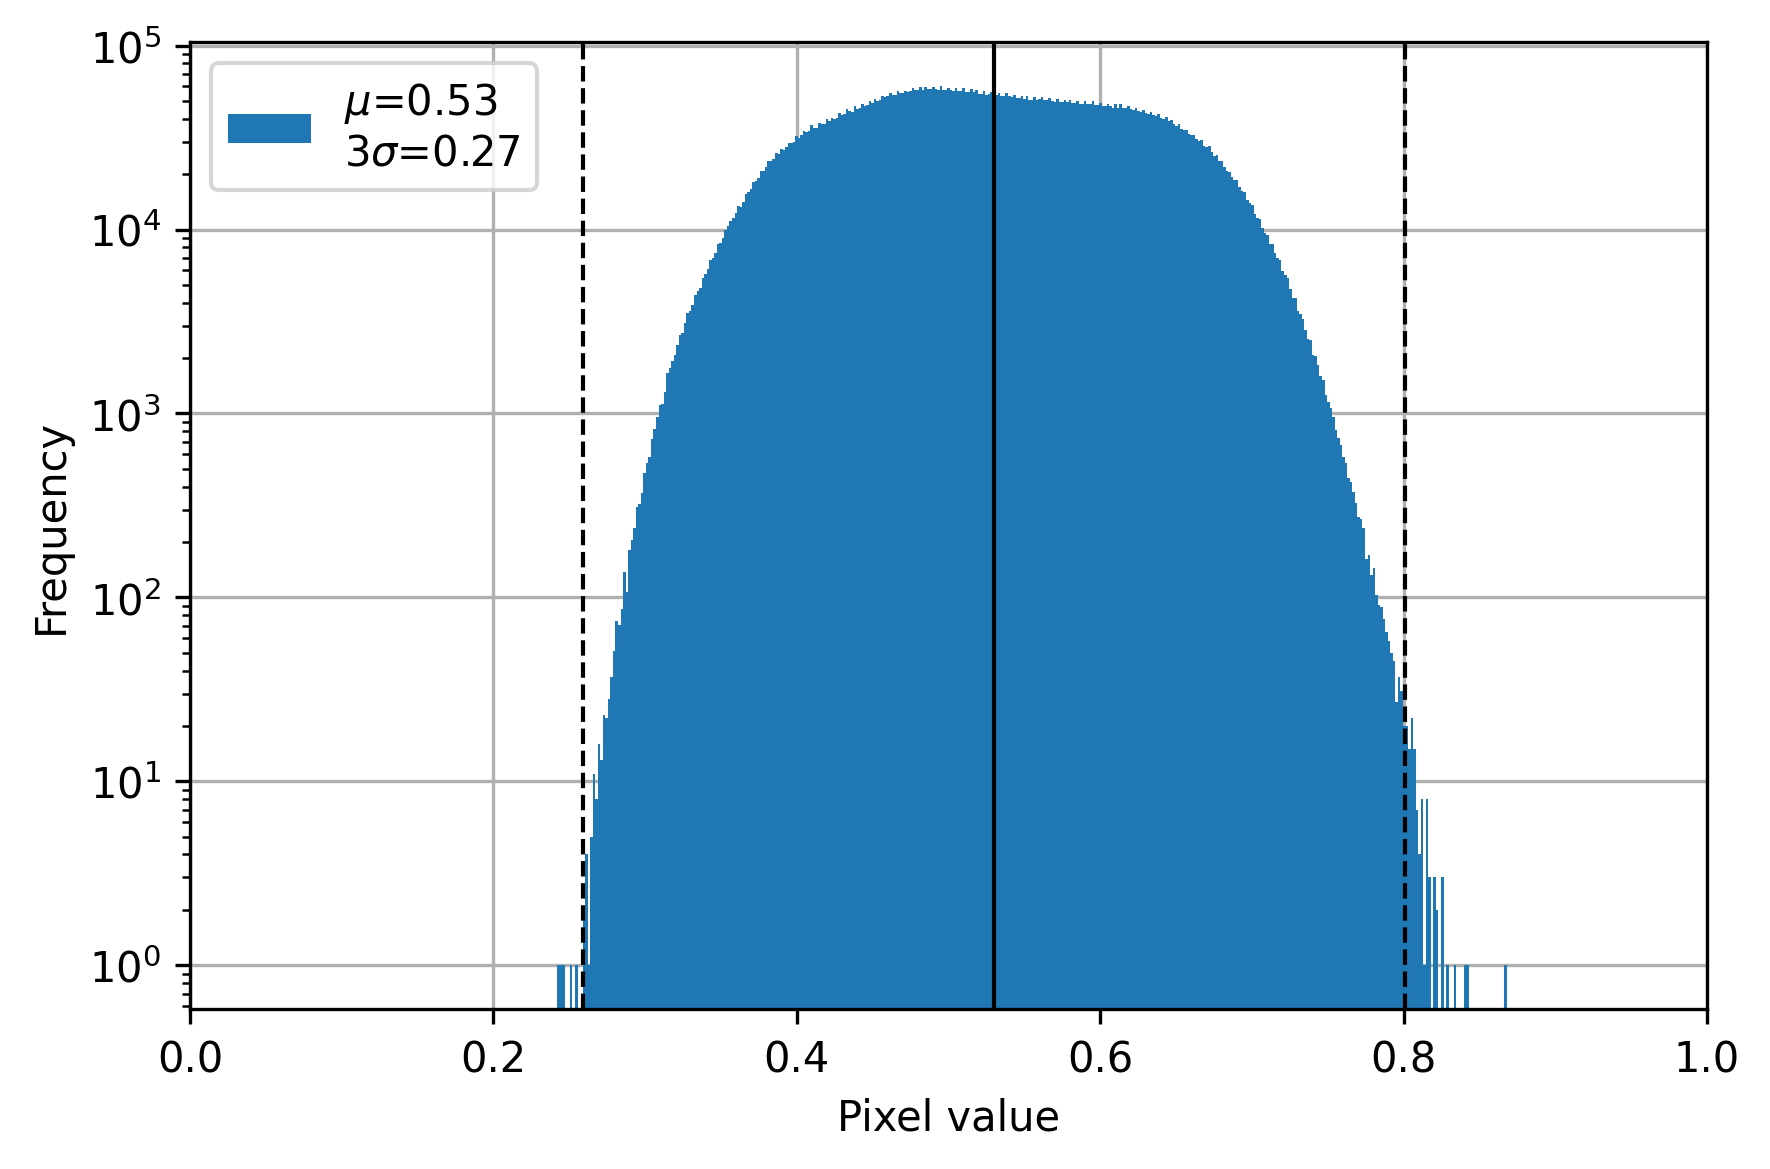
\includegraphics[width=\linewidth]{vignette-histogram.png}
    \caption{Histogram of the green channel of the white field image with relative pixel values.}
    \label{fig:vignette-histogram}
  \end{subfigure}
  \caption{}
\end{figure}

To identify faulty pixels, I compared each pixel to its neighbors in the night sky input
image. Let $I \in \mathbb{R}^{m \times n}$ be the input image and $I_{ij}$ be the
intensity of pixel $(i,j)$. I define the convolution kernel $K \in \mathbb{R}^{3 \times
    3}$ as
\begin{align*}
  K = \frac{1}{4} \begin{bmatrix}
                    1 & 0 & 1 \\
                    0 & 0 & 0 \\
                    1 & 0 & 1
                  \end{bmatrix}.
\end{align*}
Then, the mean and the standard deviation of the neighboring pixels are given by
\begin{align*}
  \mu(I)    & = I \ast K,                       \\
  \sigma(I) & = \sqrt{\mu(I^{2}) - \mu(I)^{2}},
\end{align*}
where $\ast$ denotes the convolution operation. Let $t_{\text{hot}}$ and $t_{\text{dead}}$
be thresholds for hot and dead pixels, respectively. A pixel $(i,j)$ is considered hot if
\begin{align*}
  I_{ij} > \mu(I)_{ij} + t_{\text{hot}} \cdot \sigma(I)_{ij},
\end{align*}
and dead if
\begin{align*}
  I_{ij} < \mu(I)_{ij} - t_{\text{dead}} \cdot \sigma(I)_{ij}.
\end{align*}
The thresholds can be set by the user. In my analysis, I set $t_{\text{hot}} = 3$ and
$t_{\text{dead}} = 1.2$. I chose these values by visually inspecting the images to verify
that the method correctly identifies pixels that I would consider faulty. For the input
image, this method identified 42 hot pixels and 107 dead pixels. The detected pixels are
replaced by the mean of the neighboring pixels. An example of the correction of a dead and
a hot pixel is shown in \autoref{fig:faulty-pixels}.

An alternative approach to identifying the first type of faulty pixels is to recognize
bright pixels in the black images and dark pixels in the white images. However, as can be
seen in the white image histogram in \autoref{fig:vignette-histogram} and the black image
histogram in \autoref{fig:black-histogram}, my camera did not have any permanently damaged
pixels, so I could not test this method. Also, the method described above should be able
to identify both types of faulty pixels. Therefore, I did not implement this alternative
approach.

\begin{figure}[tbp]
  \centering
  \begin{subfigure}{.49\textwidth}
    \centering
    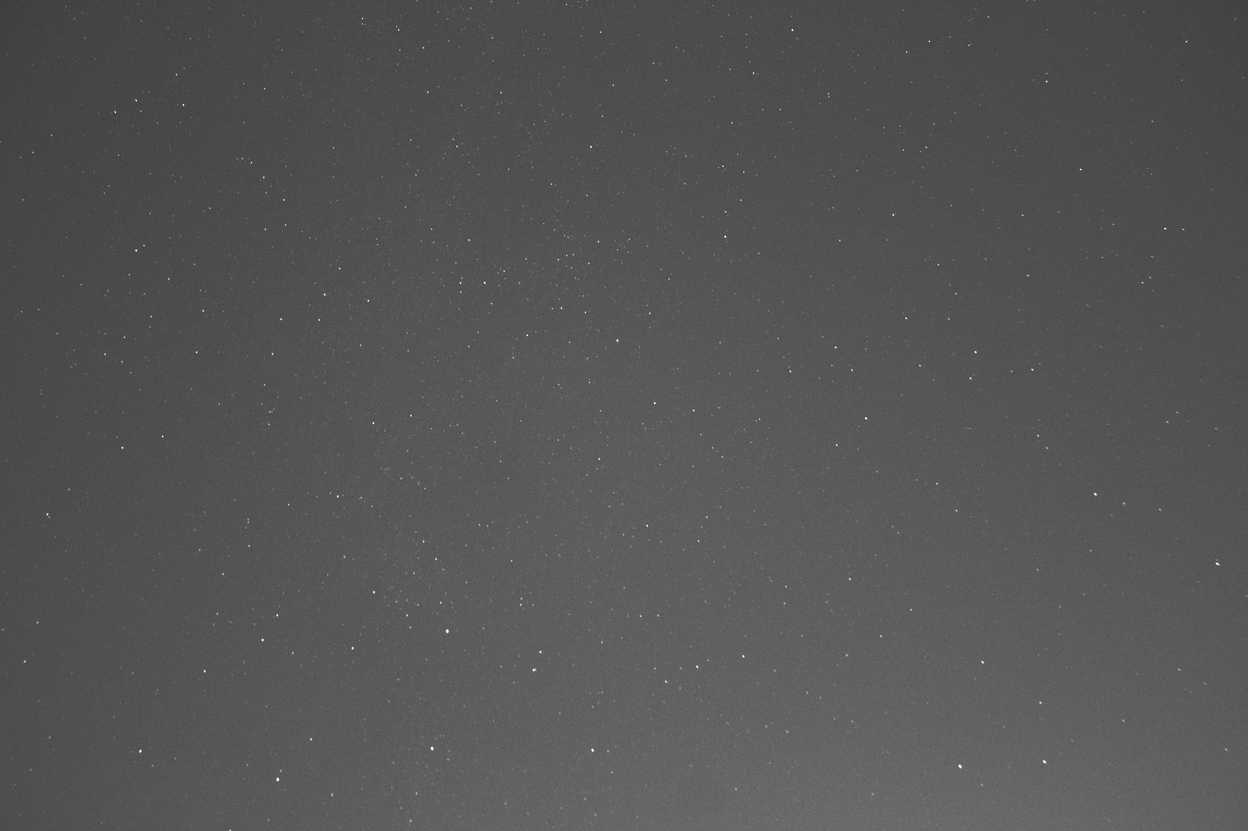
\includegraphics[width=\linewidth]{sky_green_interpolated.png}
    \caption{Before vignetting correction}
  \end{subfigure}%
  \hfill
  \begin{subfigure}{.49\textwidth}
    \centering
    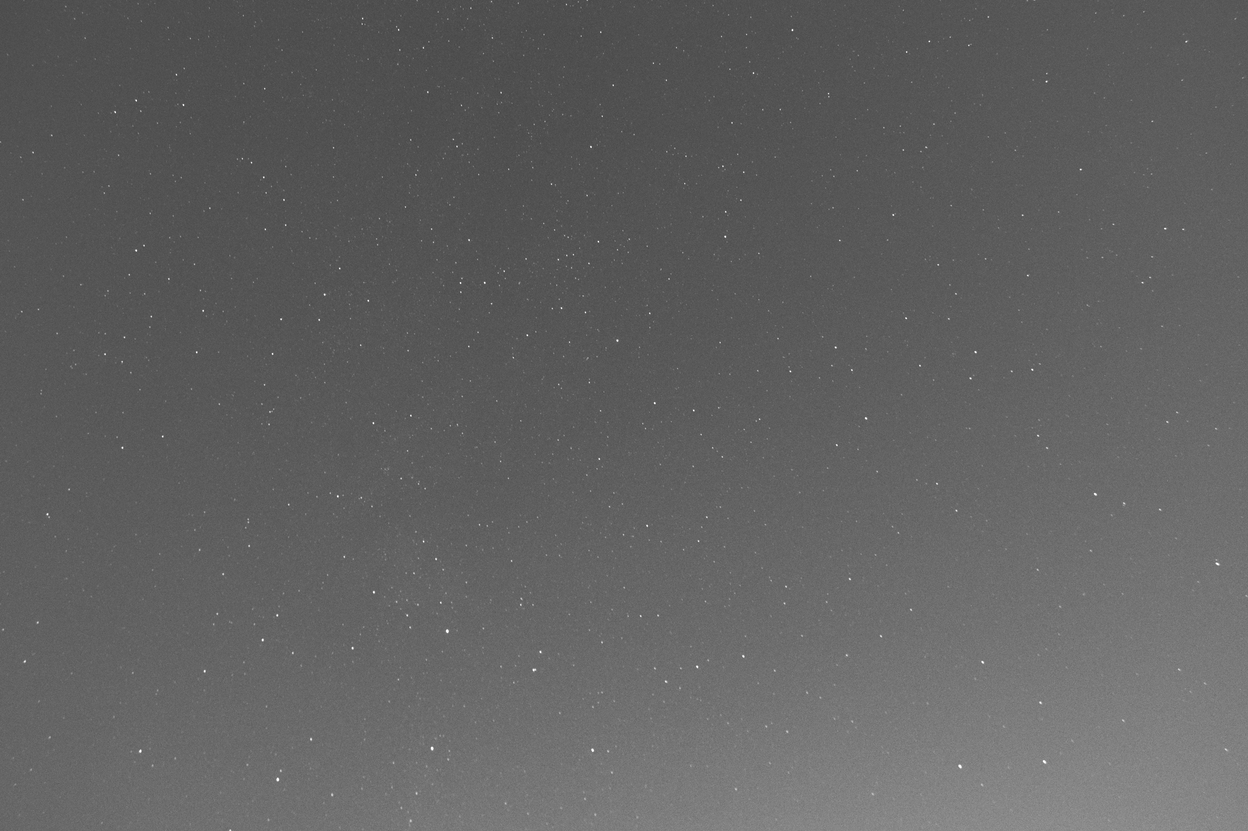
\includegraphics[width=\linewidth]{vignette_corrected.png}
    \caption{After vignetting correction}
  \end{subfigure}
  \caption{The input image before and after applying the method described in
    \autoref{sec:vignetting-correction}, interpolated for better visualization, as
    described in \autoref{sec:interpolation}.}
  \label{fig:vignette-correction}
\end{figure}

\subsection{Vignetting Correction}
\label{sec:vignetting-correction}

As light rays from the edges of the lens have to travel a longer distance to reach the
sensor, the intensity of light is lower at the edges of the image. This effect is called
vignetting and can be described by the cosine-fourth-power law. It states that the
intensity of light $B$ at an angle $\alpha$ from the center of the image is given by
\begin{align*}
  B(\alpha) = B_{0} \cdot \cos^{4}(\alpha),
\end{align*}
where $B_{0}$ is the intensity at the center of the image, assuming that the image is
distortion-free and the lens does not vignette or exhibit pupil aberrations. I correct for
this effect by dividing the input image by the white field image. Because the white field
image is homogeneously illuminated, the vignetting effect is the main feature of the
image. The white field image is shown in \autoref{fig:vignette-photo}, and its green
channel histogram is shown in \autoref{fig:vignette-histogram}. It is important that the
brightest pixels are not saturated to cover the full range of intensities. We need to
normalize the white field image, as the center of the vignette should correspond to a
correction factor of 1 and the mean and standard deviation of the distribution depend on
camera settings, like the exposure time. Therefore, we divide the white image by its
99.999th percentile, which, in this case, corresponds to the 18025th brightest pixel. This
is similar to the maximum, but more robust to outliers.

Finally, we divide the input image by the normalized white field image. The result is
shown in \autoref{fig:vignette-correction}. The vignetting effect is subtle, but visible.
In particular, the light pollution is now more pronounced in the bottom right corner,
because it was previously masked by the vignetting. I noticed that the white field image
has multiple dark spots, which are also visible in the input image, if the contrast is
increased. I cleaned the lens on the inside and outside and the mirror of the camera, but
the spots remained. I suspect that they are caused by dust on a lens element inside the
camera, which is difficult to clean without professional equipment. However, dividing by
the white field image also corrects for these spots.

\subsection{Interpolation}
\label{sec:interpolation}

As the next steps in the pipeline require a complete image, we need to interpolate the
missing pixels. Iterating over the pixels separately would take several seconds for an
image of this size, so I used a convolution with the following kernel instead.
\begin{align*}
  K = \frac{1}{4} \begin{bmatrix}
                    0 & 1 & 0 \\
                    1 & 0 & 1 \\
                    0 & 1 & 0
                  \end{bmatrix}.
\end{align*}
Each missing pixel is replaced by the corresponding pixel in the convolution of the input
image with the kernel. The result is shown in \autoref{fig:interpolation}.

\begin{figure}[tb]
  \centering
  \begin{subfigure}{.33\textwidth}
    \centering
    
\includegraphics[width=\linewidth]{raw_cutout.png}
    \caption{Raw image}
  \end{subfigure}%
  \hfill
  \begin{subfigure}{.33\textwidth}
    \centering
    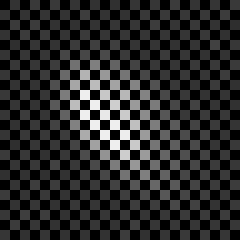
\includegraphics[width=\linewidth]{green_only_cutout.png}
    \caption{After masking}
  \end{subfigure}%
  \hfill
  \begin{subfigure}{.33\textwidth}
    \centering
    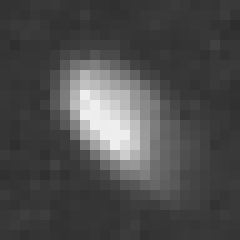
\includegraphics[width=\linewidth]{green_interpolated_cutout.png}
    \caption{After interpolation}
  \end{subfigure}
  \caption{A cutout of the input image, comparing it at different stages of the pipeline.}
  \label{fig:interpolation}
\end{figure}


\subsection{Skyglow Correction}
\label{sec:skyglow-correction}

Another common source of noise in night sky images is light pollution from artificial
sources, like street lamps or buildings. This light is reflected by particles in the
atmosphere and causes a bright background in the image. I refer to this effect as skyglow.
It appears as a smooth gradient in the image with no hard edges or localized features.
Stars, on the other hand, are point sources of light and have a sharp intensity profile.
Therefore, we can correct for skyglow by subtracting a smoothed version of the image from
the original image.

To smooth the image, I used a Gaussian filter with a kernel size of $700 \times 700$
pixels and a standard deviation of 200 pixels. The kernel size is chosen to be large, so
that all stars are fully smoothed out. The smoothed image is shifted by subtracting its
minimum pixel value to avoid negative values. The corrected image is then obtained by
subtracting the smoothed image from the input image and clipping the result to the range
$[0, 16383]$.

The blurred image and the result of the skyglow correction are shown in
\autoref{fig:skyglow}. The gradient in the blurred image shows lines instead of a smooth
gradient. This is because the original blurred image is very dim and, to show it in this
paper, I converted it to 8-bit and increased the contrast and brightness. As the original
image is 14-bit, the lines are not visible there. After correction, the background of the
processed image is much more uniform. However, this method is only beneficial for
wide-field images with no obstructing objects. If there are trees, buildings or the moon
in the image, subtracting the blurred image might worsen the magnitude estimation near the
objects. Also, in images with a narrow field of view, the skyglow is much more uniform,
making the method unnecessary. The user can disable the skyglow correction in these cases.

\begin{figure}[tb]
  \centering
  \begin{subfigure}{.49\textwidth}
    \centering
    
\includegraphics[width=\linewidth]{skyglow_blurred.png}
    \caption{Input image after blurring, adjusted for better visualization.}
    \label{fig:skyglow-blurred}
  \end{subfigure}%
  \hfill
  \begin{subfigure}{.49\textwidth}
    \centering
    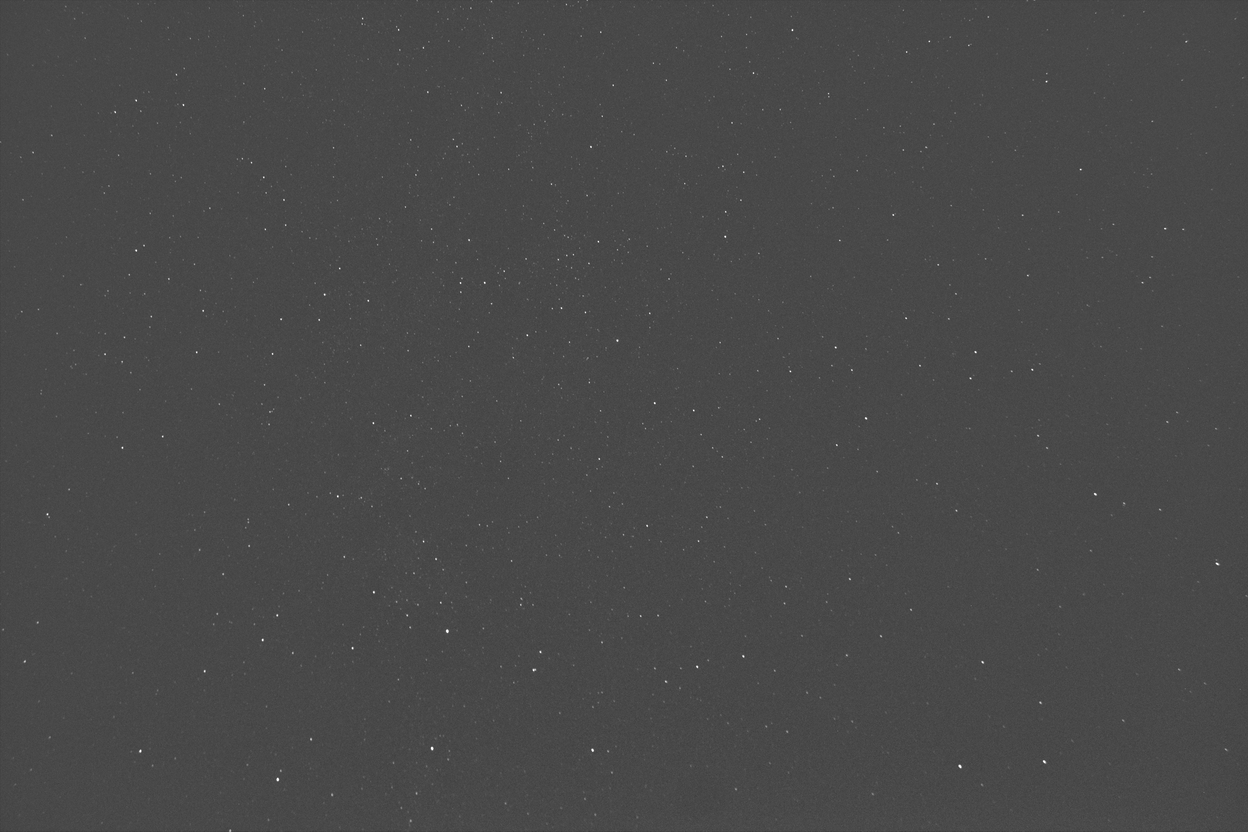
\includegraphics[width=\linewidth]{skyglow_corrected.png}
    \caption{The processed image after skyglow correction.\\\text{}}
    \label{fig:skyglow-corrected}
  \end{subfigure}
  \caption{Skyglow correction, see \autoref{sec:skyglow-correction}}
  \label{fig:skyglow}
\end{figure}

\subsection{Full Pre-Processing Pipeline}
\label{sec:full-pipeline}

The previous sections describe the major steps of the pre-processing pipeline. An overview
of the order of the steps and how they are applied to the input image is shown in
\autoref{fig:full-pipeline}. The pipeline takes a raw night sky image, a black field image
and a white field image as input. The red and blue channels of all images are masked (not
shown in the figure for simplicity). After the faulty pixels are corrected, the mean of
the black image is subtracted from the input image and the result is clipped to the range
$[0, 16383]$. This reduces the noise in the dark pixels because every pixel with a value
below the mean of the black image is set to 0. The next steps are the vignetting
correction, interpolation and skyglow correction, as described in the previous sections.
Lastly, the image is normalized by dividing it by its maximum pixel value. I assume that
at least some pixels in the image are saturated. However, different cameras saturate at
different values and the previous steps might have reduced the values of the brightest
pixels. Also, the bit depth would affect the analysis results, if it would use absolute
pixel values. Therefore, I normalize the image to the range $[0, 1]$ to get consistent
results across different cameras and bit depths. The output of the pipeline is a
pre-processed image that can be used for further analysis. I will refer to this image as
the \textit{calibrated image} in the following sections. Histograms of the pixel values of
the input and output images are shown in \autoref{fig:input-output}. Each step of the
pipeline can be disabled by the user, if it is not necessary for the specific image.

\begin{figure}[tbp]
  \centering
  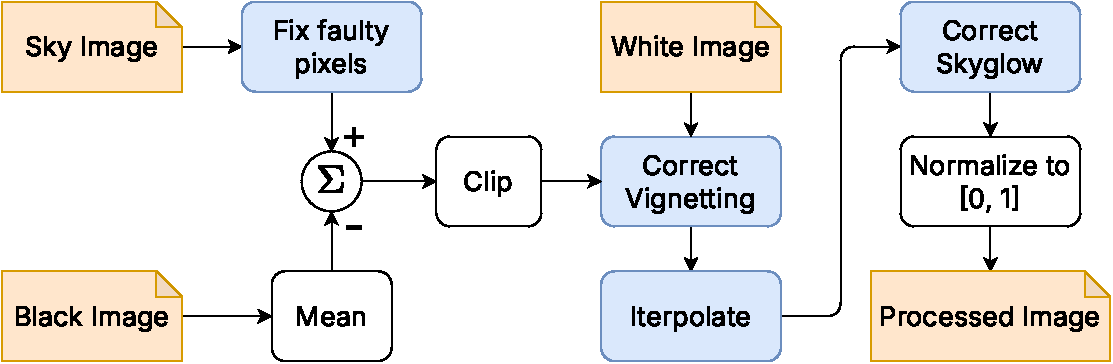
\includegraphics[width=\linewidth]{full_pipeline.pdf}
  \caption{The full pre-processing pipeline for the input image.}
  \label{fig:full-pipeline}
\end{figure}

\begin{figure}[tbp]
  \centering
  \begin{subfigure}{.49\textwidth}
    \centering
    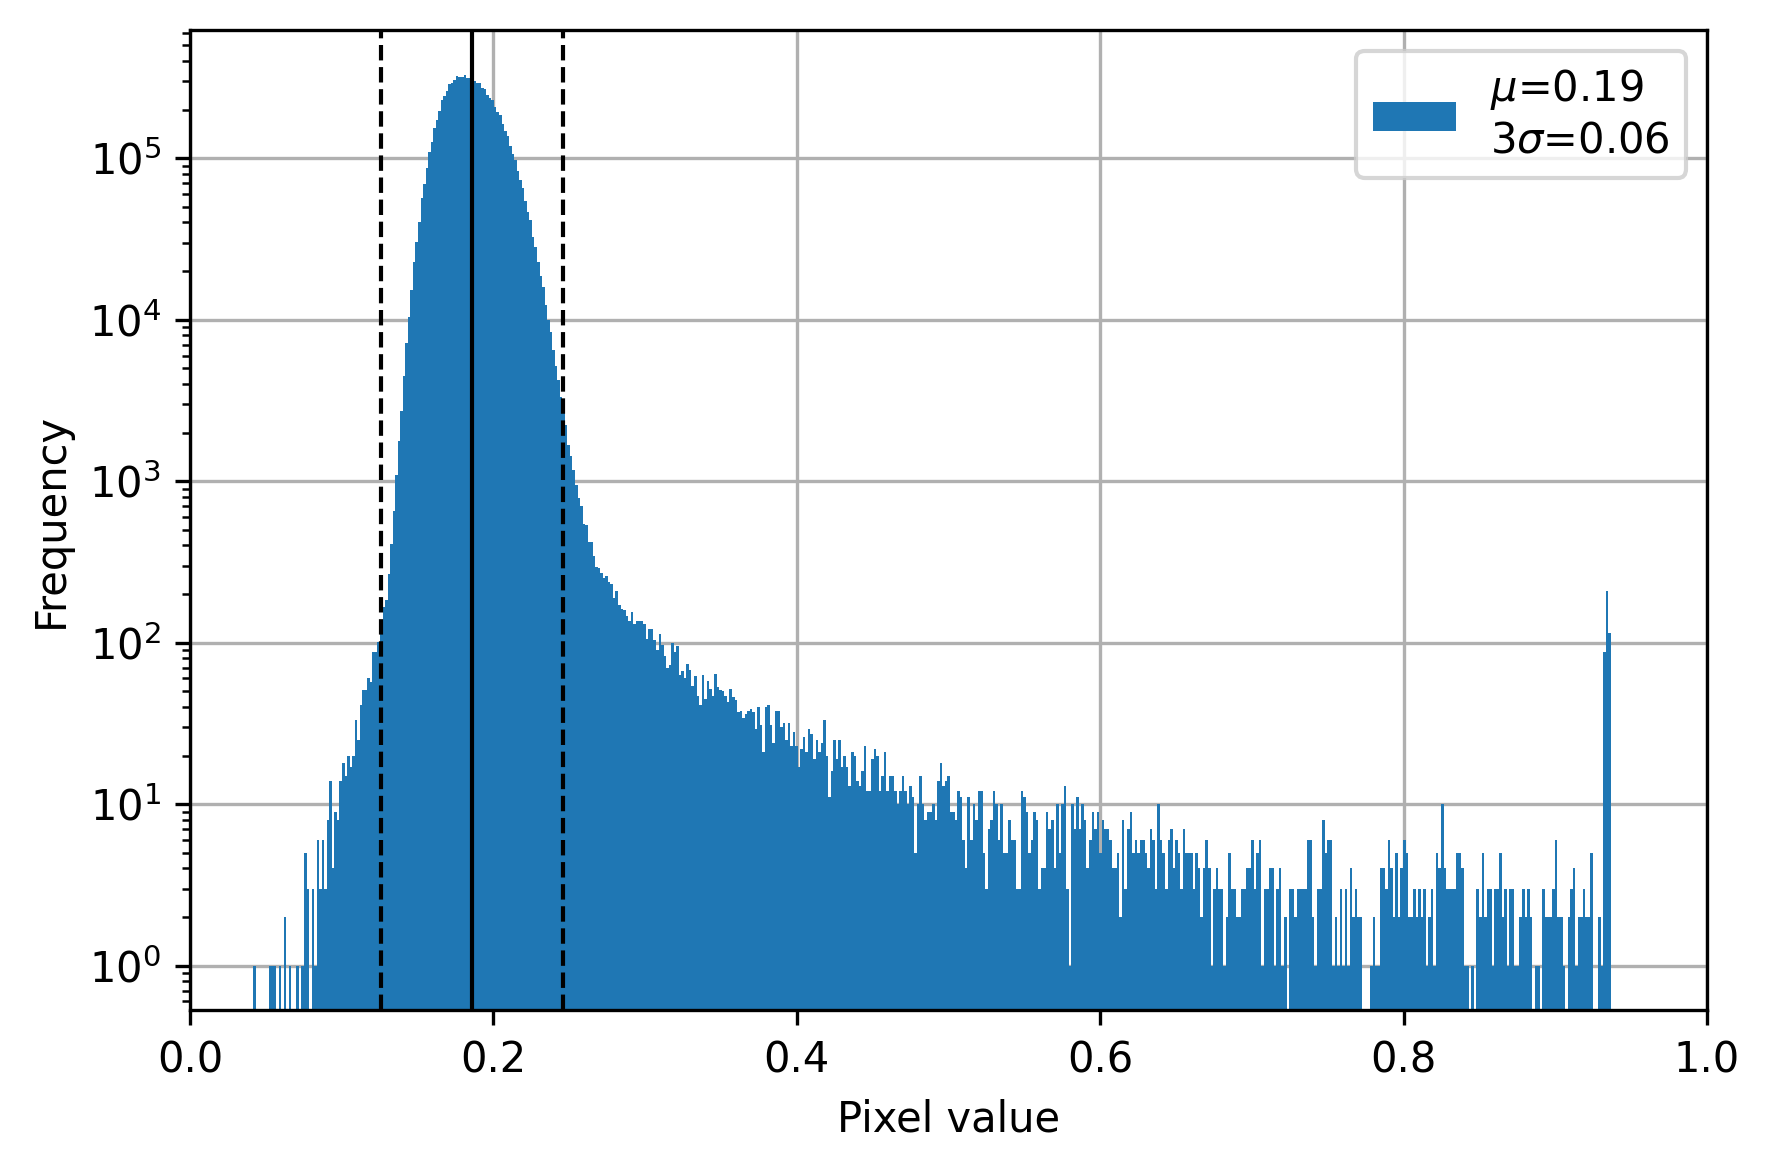
\includegraphics[width=\linewidth]{histogram_input.png}
    \caption{Input image}
    \label{fig:pipeline-input}
  \end{subfigure}%
  \hfill
  \begin{subfigure}{.49\textwidth}
    \centering
    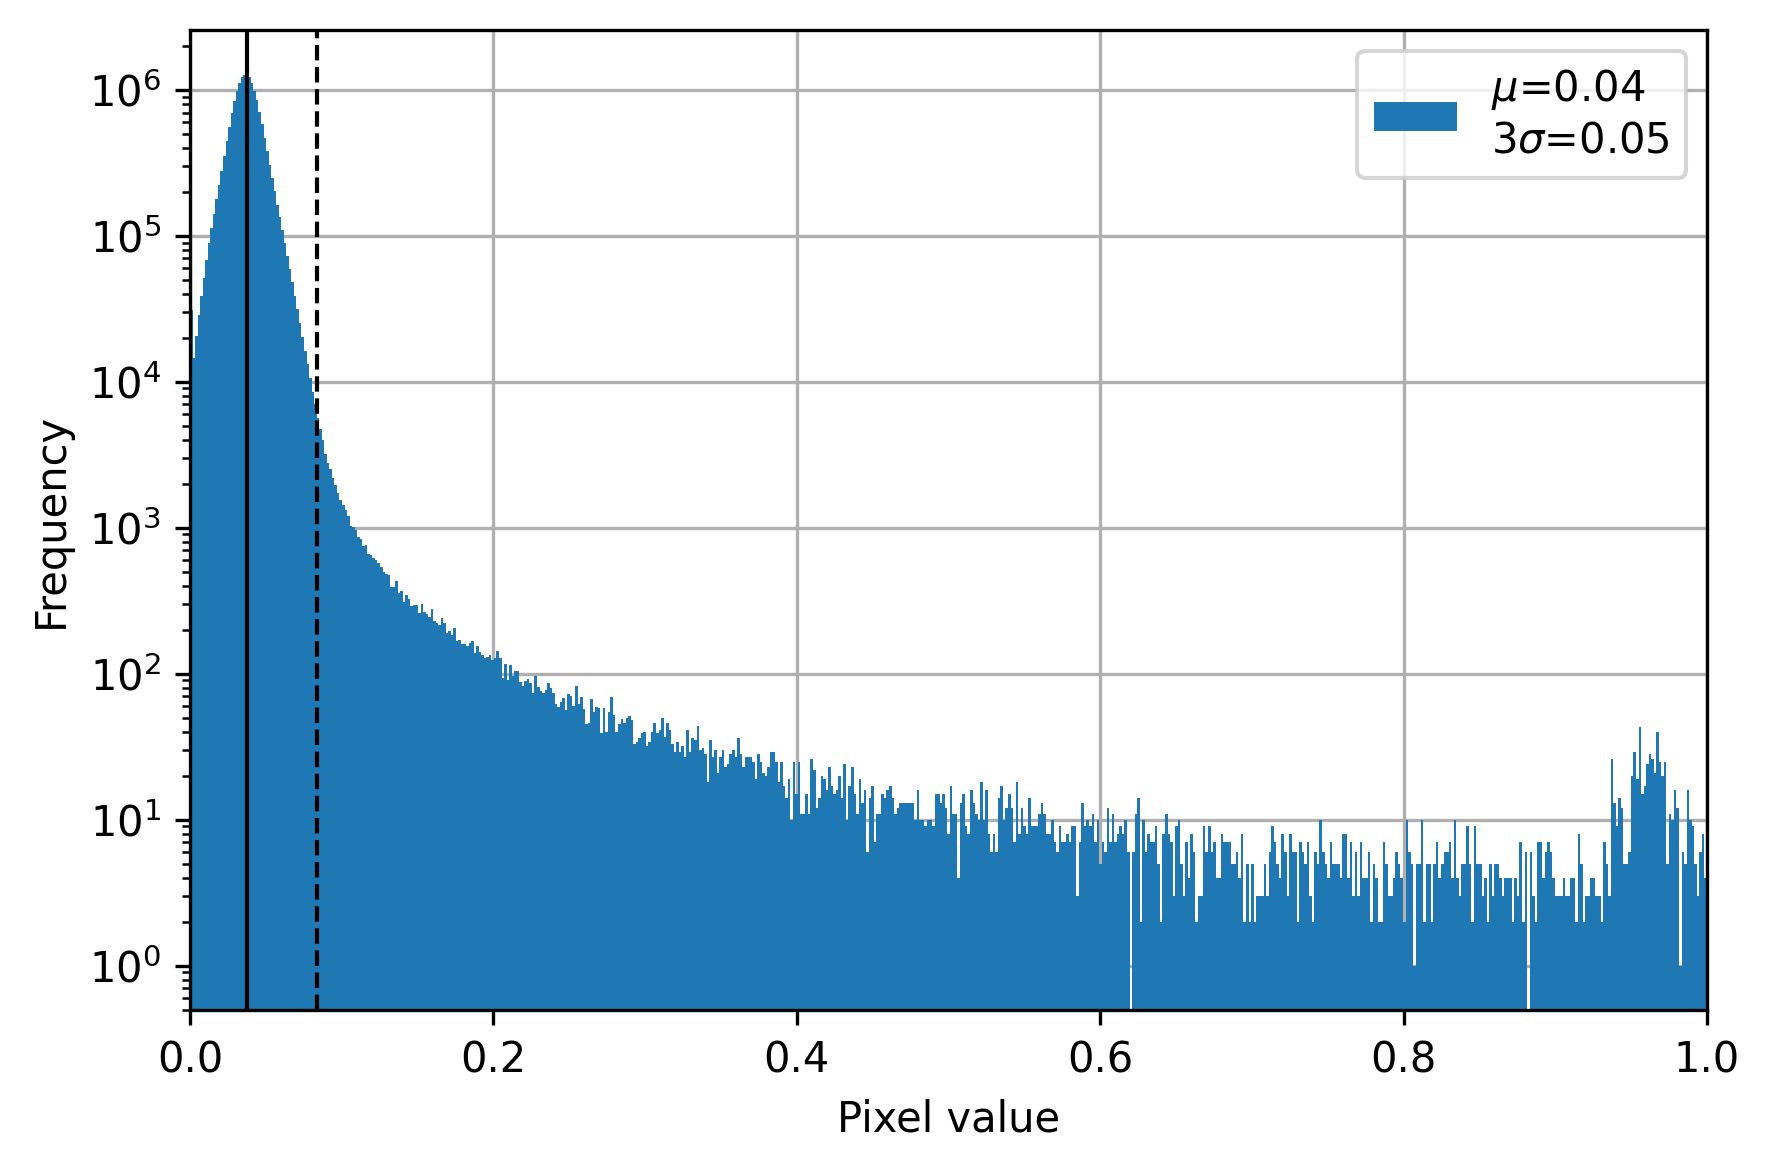
\includegraphics[width=\linewidth]{histogram_output.png}
    \caption{Output image}
    \label{fig:pipeline-output}
  \end{subfigure}
  \caption{Histograms of the input and output images of the full pre-processing pipeline.}
  \label{fig:input-output}
\end{figure}


\section{Analysis}
\label{sec:analysis}

The main goal of the analysis is to estimate the source-count distribution of stars in the
images by predicting their magnitudes. I fitted a model to the input image, which can be
used by the user to predict the magnitudes of stars in other images. To train the
predictor, I needed to obtain the true magnitudes of stars in the input image. This
process involves multiple steps, that can be used independently. The first step finds the
pixel coordinates of each star in the image (\autoref{sec:star-identification}). These are
mapped to the celestial sphere to find the corresponding right ascension and declination
(\autoref{sec:pixel-to-sky-mapping}). The true magnitudes are obtained by matching the
sky coordinates to stars in the SIMBAD database (\autoref{sec:catalog-matching}). The
model is then fitted to the labeled list of stars (\autoref{sec:magnitude-estimation}).
Finally, the distribution of predicted magnitudes is compared to the literature
(\autoref{sec:source-count-distribution}).

\subsection{Star Identification}
\label{sec:star-identification}

\begin{figure}[tb]
  \centering
  \begin{subfigure}{.33\textwidth}
    \centering
    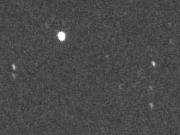
\includegraphics[width=\linewidth]{floodFill_original.png}
    \caption{Cutout of the input image}
    \label{fig:floodfill-original}
  \end{subfigure}%
  \hfill
  \begin{subfigure}{.33\textwidth}
    \centering
    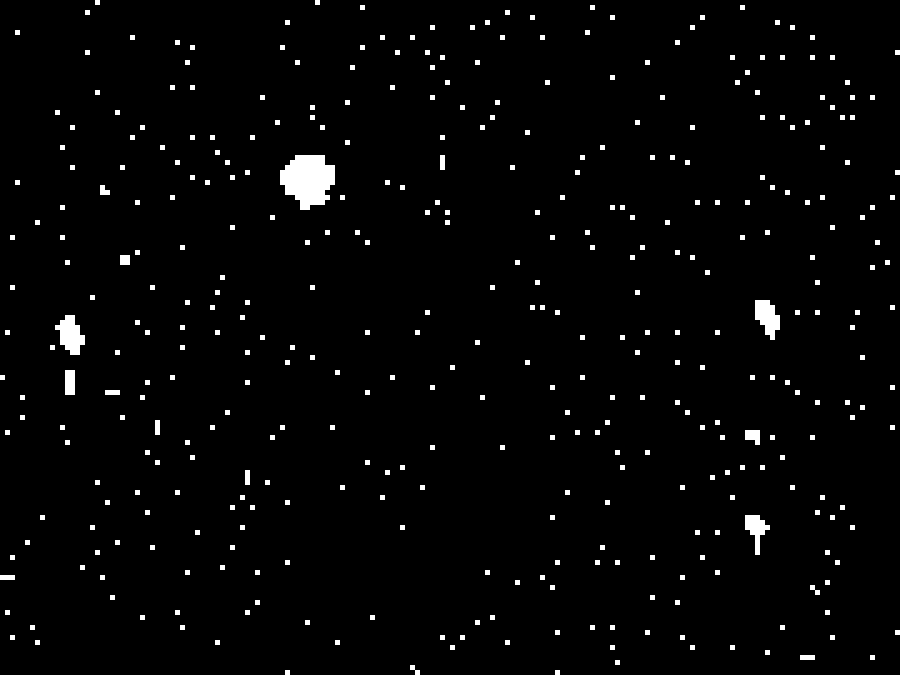
\includegraphics[width=\linewidth]{floodFill_before_erode.png}
    \caption{Mask after \texttt{floodFill} method}
    \label{fig:floodfill}
  \end{subfigure}%
  \hfill
  \begin{subfigure}{.33\textwidth}
    \centering
    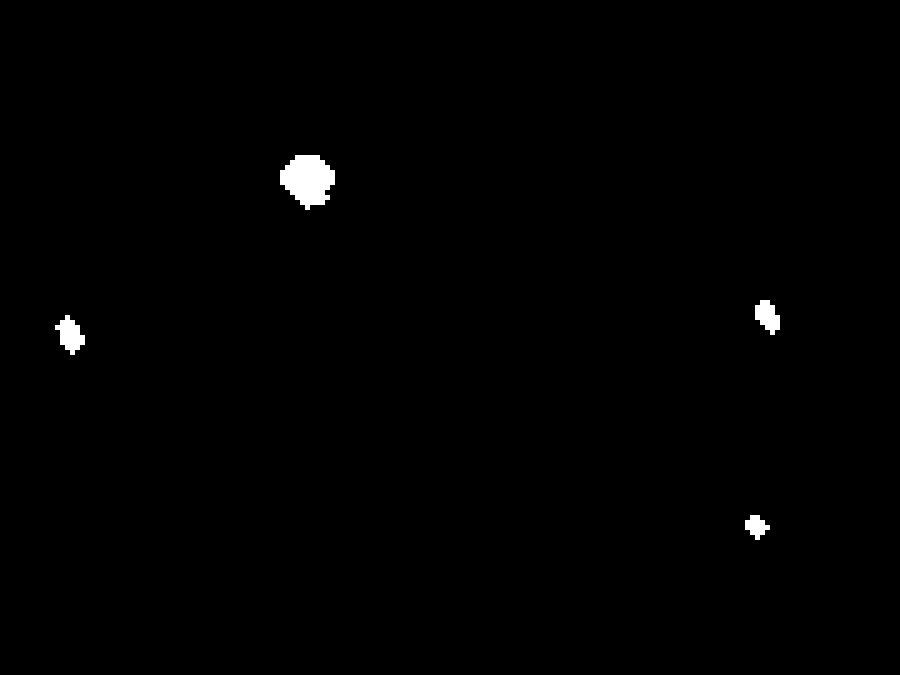
\includegraphics[width=\linewidth]{floodFill_after_erode.png}
    \caption{Mask after Opening operation}
    \label{fig:opening}
  \end{subfigure}
  \caption{}
  \label{fig:star-identification}
\end{figure}

Starting from the calibrated image, we need to identify the stars in the image. First,
we classify each pixel as belonging to a star or the background. A fast and simple
approach is the \texttt{cv2.floodFill} method from the OpenCV library \cite{opencv2000}.
It starts at a seed pixel, fills all connected pixels with a similar intensity and returns
the mask of the filled area. A pixel $(x, y)$ with a value $\texttt{src}(x, y)$ is
considered to have a similar intensity iff
\begin{align*}
  \texttt{src}(x', y') - \texttt{loDiff} \leq \texttt{src}(x, y) \leq \texttt{src}(x', y') + \texttt{upDiff},
\end{align*}
where $\texttt{src}(x', y')$ is the value of one of the neighboring pixels that is already
filled and \texttt{loDiff} and \texttt{upDiff} are thresholds set by the user. This rule
is applied iteratively to all pixels. To fill the background of the input image, I
chose the darkest pixel as the seed and set $\texttt{loDiff} = \infty$ and
$\texttt{upDiff} = 5$ (for an 8-bit image). A lower value of \texttt{upDiff} would result
in too much noise being classified as stars, while a higher value would miss faint stars.
The result is shown in \autoref{fig:floodfill}. We can see that there are many single
pixels of noise not being classified as background. To remove them, I applied the
morphological operation Opening with a $3 \times 3$ kernel using the
\texttt{cv2.morphologyEx} method from OpenCV. This operation erodes the image and then
dilates it, which removes objects that are at most two pixels wide. All other components
are preserved. The result is shown in \autoref{fig:opening}. Finally, I used the
\texttt{cv2.connectedComponents} method to separate the objects in the mask. I defined the
center of the bounding box of each object as the pixel coordinates of the star it
corresponds to.

In the calibrated image, the method identified 1001 stars. According to the SIMBAD
database, there are 746 stars with a visible magnitude of less than 7.0 and 2330 stars
with a magnitude less than 8.0 in the field of view of the image. The ADQL query used to
obtain this number is given in \autoref{lst:simbad-query}. If two stars are very close
together, the method might classify them as one object. During visual inspection however,
I only found two cases of this happening. Stars not being recognized is more commonly due
to them being too faint to distinguish them from noise. \autoref{fig:removing-stars} shows
histograms of the calibrated image before and after removing the stars identified by this
method. In \autoref{fig:after-removing-stars} we can see that almost all pixels identified
as background have a relative value of at most $20\%$.

I also tested other approaches, like template matching. The main problem was to define a
general template for stars, that would fit different sizes and brightnesses. This drawback
made template matching much more complex and less reliable than the flood fill method.

\begin{figure}[tb]
  \centering
  % \begin{subfigure}{.33\textwidth}
  %   \centering
  %   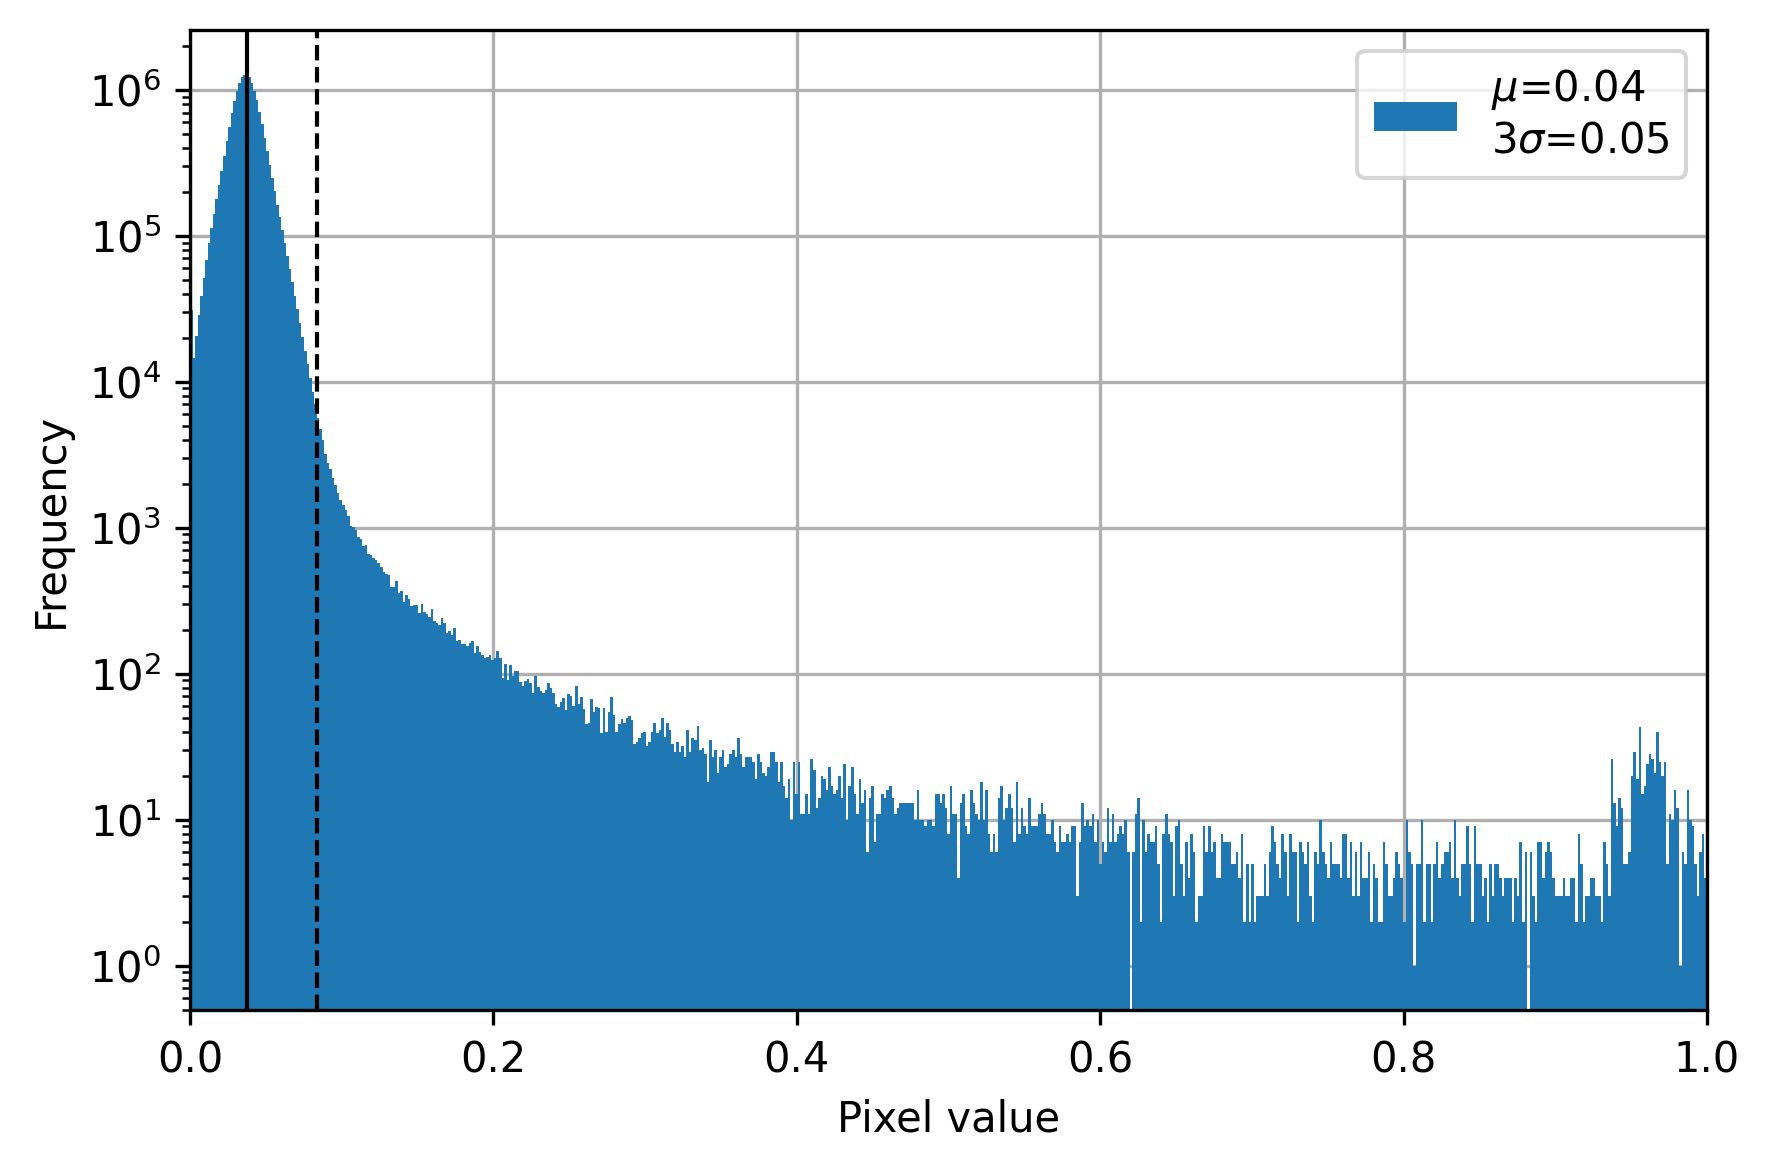
\includegraphics[width=\linewidth]{histogram_output.png}
  %   \caption{Calibrated image\\\text{}}
  %   \label{fig:before-removing-stars}
  % \end{subfigure}%
  % \hfill
  \begin{subfigure}{.49\textwidth}
    \centering
    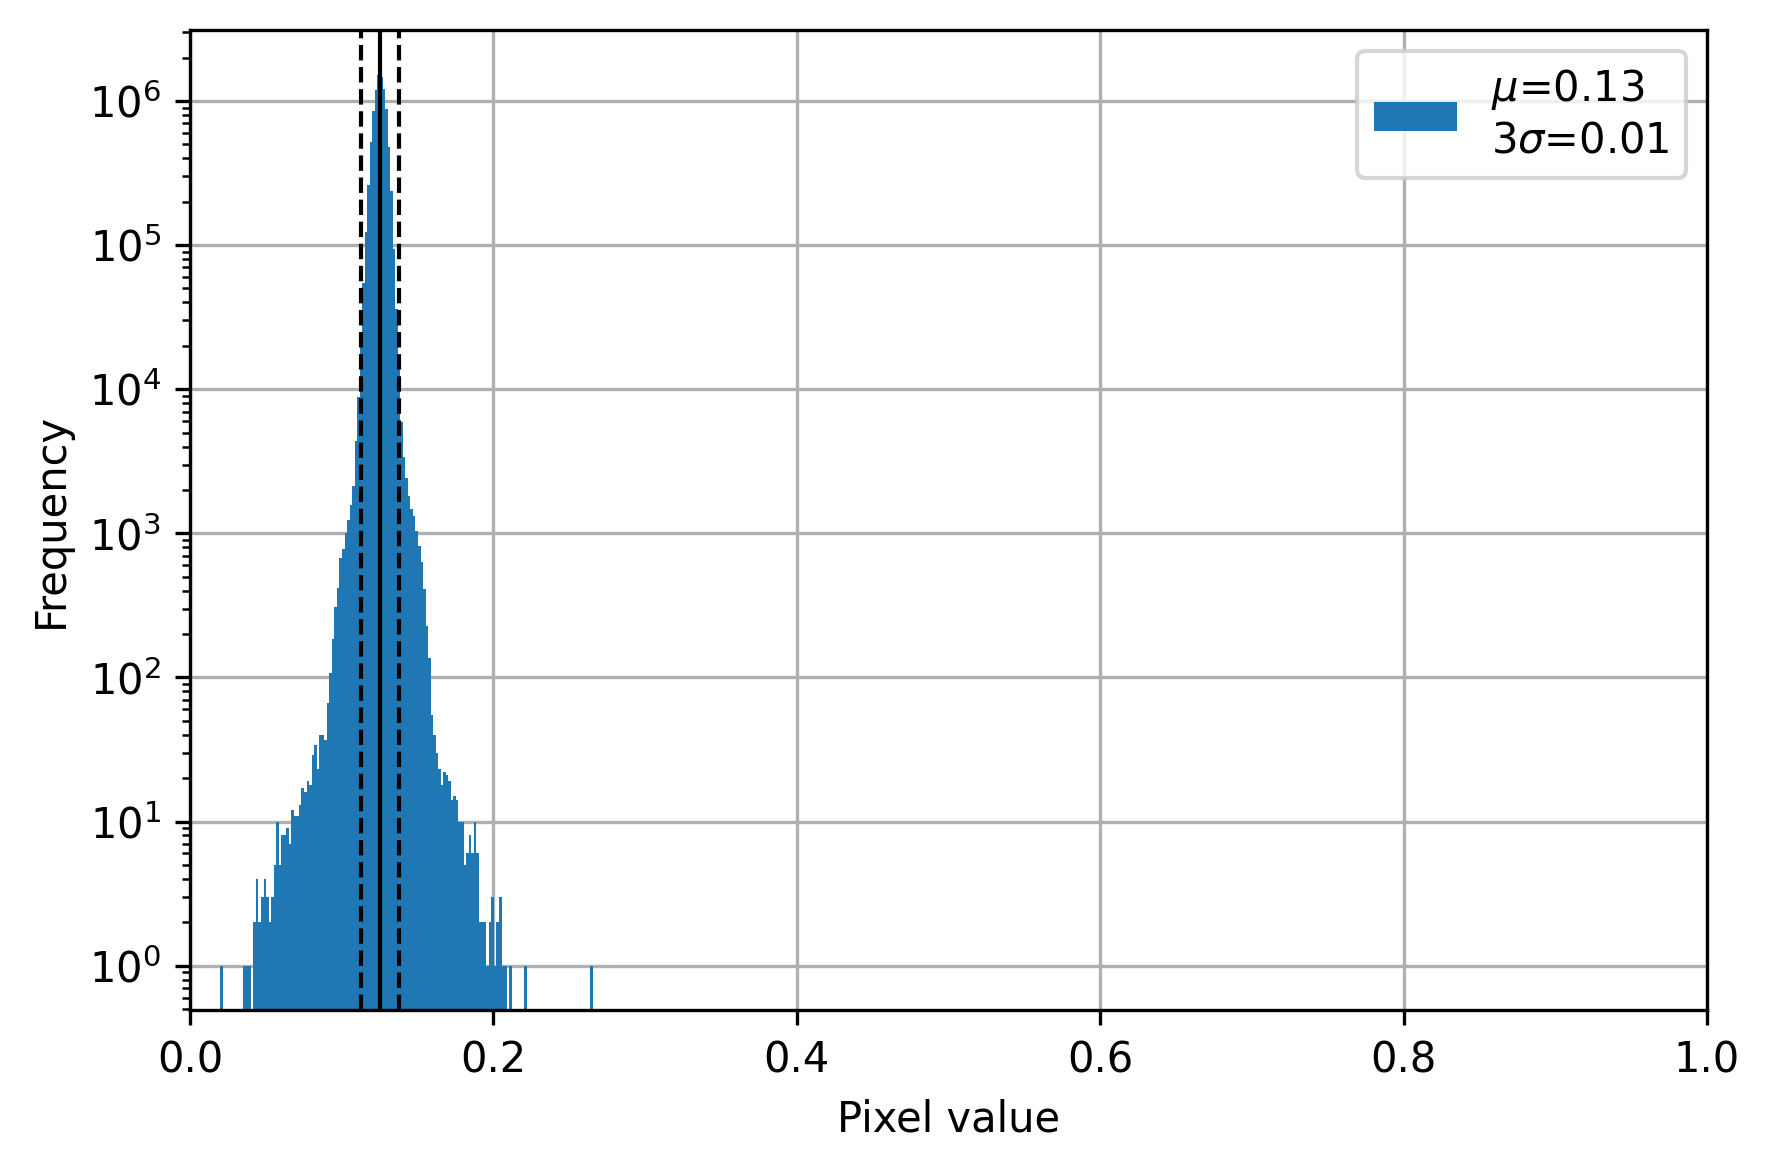
\includegraphics[width=\linewidth]{histogram_black_single.png}
    \caption{Black image taken with the lens cap on, not normalized.}
    \label{fig:black-histogram}
  \end{subfigure}%
  \hfill
  \begin{subfigure}{.49\textwidth}
    \centering
    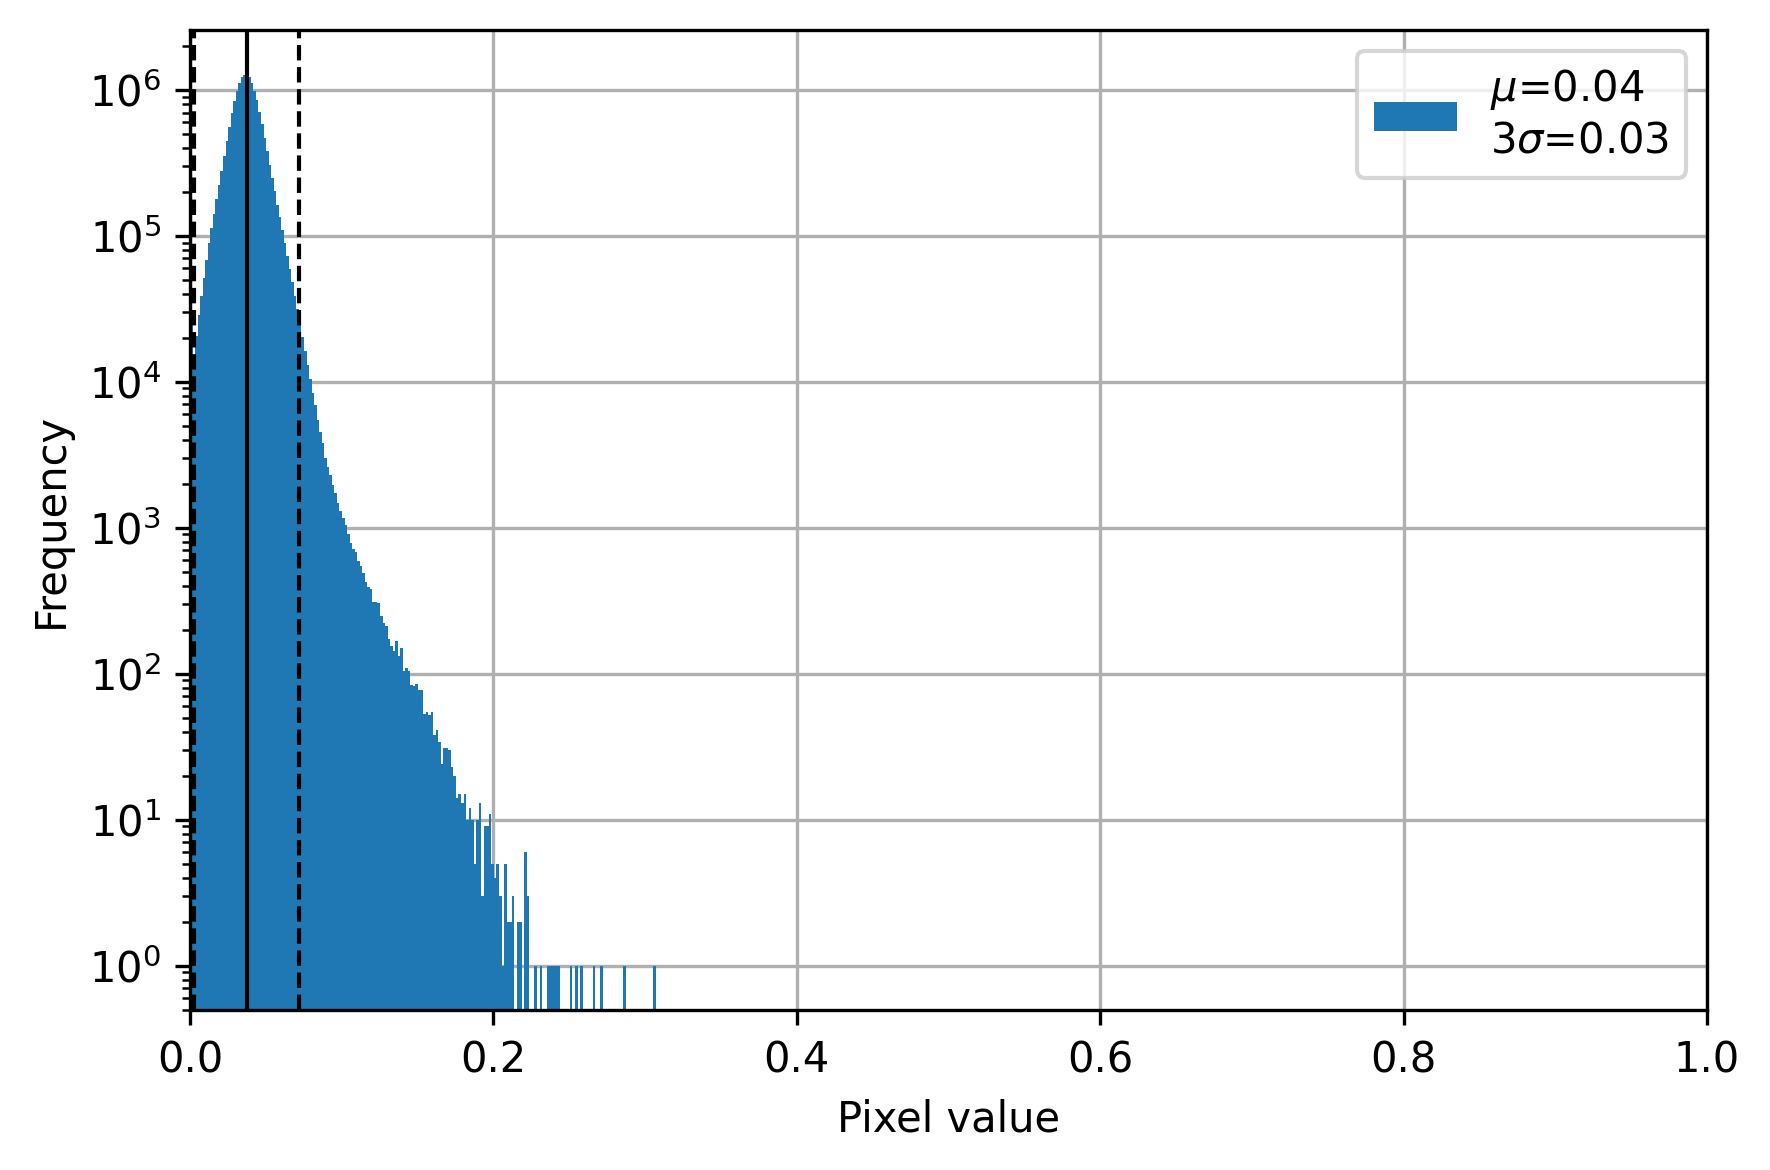
\includegraphics[width=\linewidth]{histogram_no_stars.png}
    \caption{After removing all star-pixels found by the method in \autoref{sec:star-identification}.}
    \label{fig:after-removing-stars}
  \end{subfigure}
  \caption{}
  \label{fig:removing-stars}
\end{figure}

\subsection{Pixel to Sky Mapping}
\label{sec:pixel-to-sky-mapping}

To find the true magnitude of a star in the input image, we need to know its right
ascension and declination. This requires mapping the pixel coordinates of the star to the
celestial sphere. Therefore, we need to know the orientation of the camera and the field
of view of the lens. The website
\href{https://nova.astrometry.net}{\texttt{astrometry.net}} \cite{astrometry2010} allows
users to upload an image and returns the world coordinates of the center of the image and
other helpful information. An upload of the input image is linked and shown in
\autoref{fig:astrometry-output}. However, as the \texttt{brightest} library is meant to be
used without manual intervention or an internet connection, I used the \texttt{astrometry}
Python library, which only includes the algorithm for astrometric plate solving used by
the website. Given a set of pixel coordinates and limits for the field of view, the
\texttt{astrometry} library returns an \texttt{astropy.WCS} (World Coordinate System)
object, which can be used to map pixel to world coordinates.

The solver tries to find the best match between the input coordinates and a catalog of
stars. I used the recommended built-in dataset based on a subset of the Tycho-2 catalog,
available at \href{http://data.astrometry.net/4100/}{\texttt{data.\allowbreak
    astro\allowbreak metry.\allowbreak net}}. Additionally, the solver is given a lower and
upper limit for the scale of the image, expressed in arcseconds per pixel. My camera has a
sensor size of $x \times y = 22.3 \times 14.9$ mm and a focal length of $f = 18$. Then
field of view is given by
\begin{align*}
  \text{FOV}_x & = 2 \arctan{\left(\frac{x}{2f}\right)} = 63.55^\circ  \\
  \text{FOV}_y & = 2 \arctan{\left(\frac{y}{2f}\right)} = 44.97^\circ.
\end{align*}
With a horizontal resolution of 5202 pixels, we get $\text{scale} = \text{FOV}_x / 5202 =
  43.98$ arcsec/pixel. For the input image (\autoref{fig:sky-input}), the solver located
the center of the image at right ascension $20^\text{h}\ 50^\text{m}\ 49.81^\text{s}$
and declination $+60^\circ\ 10'\ 15.02''$. An annotated version of the image, showing
the constellations, is shown in \autoref{fig:astrometry-output}. Using the returned
\texttt{astropy.WCS} object, the pixel coordinates of the stars are transformed to sky
coordinates.

\subsection{Catalog Matching}
\label{sec:catalog-matching}

Now that we know the sky coordinates of the stars in the input image, we can match them
to stars in a catalog provided by the user. As mentioned in
\autoref{sec:pixel-to-sky-mapping}, the \texttt{astrometry} library already provides a
built-in catalog. However, it is only a small subset of the Tycho-2 data so that the
solver can run quickly.

Instead, I queried the SIMBAD database \cite{Wenger_2000}. It is one of the most
comprehensive astronomical databases and presently contains information on about 8.9
million stars and 9.3 million non-stellar objects. I queried the database for stars with a
visible magnitude of less than 8.0 in the field of view of the input image. Visual
inspection showed that stars with a higher magnitude were not distinguishable from noise
in the calibrated image. For other images, the maximum magnitude can be set by the user.

Matching the star positions is done by calling the \texttt{SkyCoord.\allowbreak
  match\_to\_catalog\_sky} method from the \texttt{astropy} library \cite{astropy2022} with
the sky coordinates of the stars in the image and the catalog. It constructs a KD-Tree
from the catalog and performs a nearest-neighbor search for each star in the image. The
result is an index map that assigns a catalog star to each star in the image. The accuracy
of this method depends mostly on the accuracy of the solution of the astrometric plate
solver (\autoref{sec:pixel-to-sky-mapping}). The more the coordinates are off, the higher
the chance that the nearest neighbor is not the correct match. Therefore, it is important
to use a conservative maximum magnitude for the SIMBAD query to keep the size of the
catalog close to the number of stars in the image.

\subsection{Magnitude Estimation}
\label{sec:magnitude-estimation}

\begin{figure}[tb]
  \centering
  \begin{subfigure}{.49\textwidth}
    \centering
    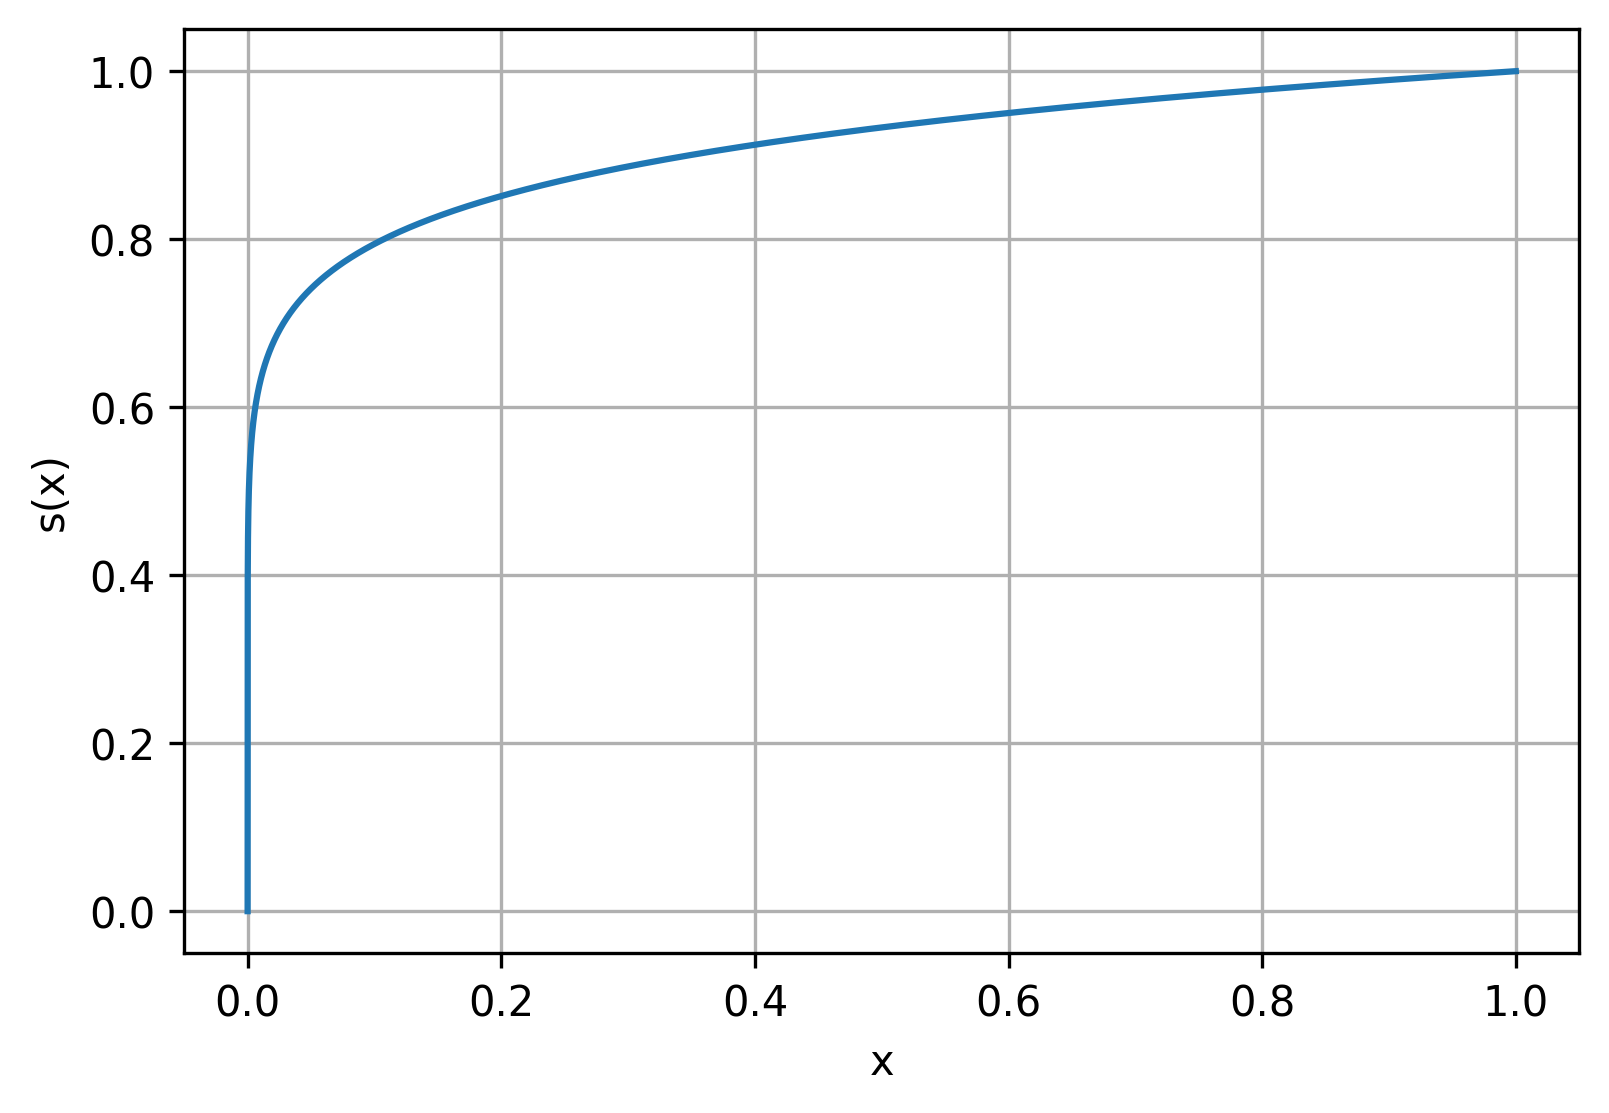
\includegraphics[width=\linewidth]{x_pow_0.1.png}
    \caption{Scaling function $s(x) = x^{0.1}$}
    \label{fig:kmeans-scaling}
  \end{subfigure}%
  \hfill
  \begin{subfigure}{.49\textwidth}
    \centering
    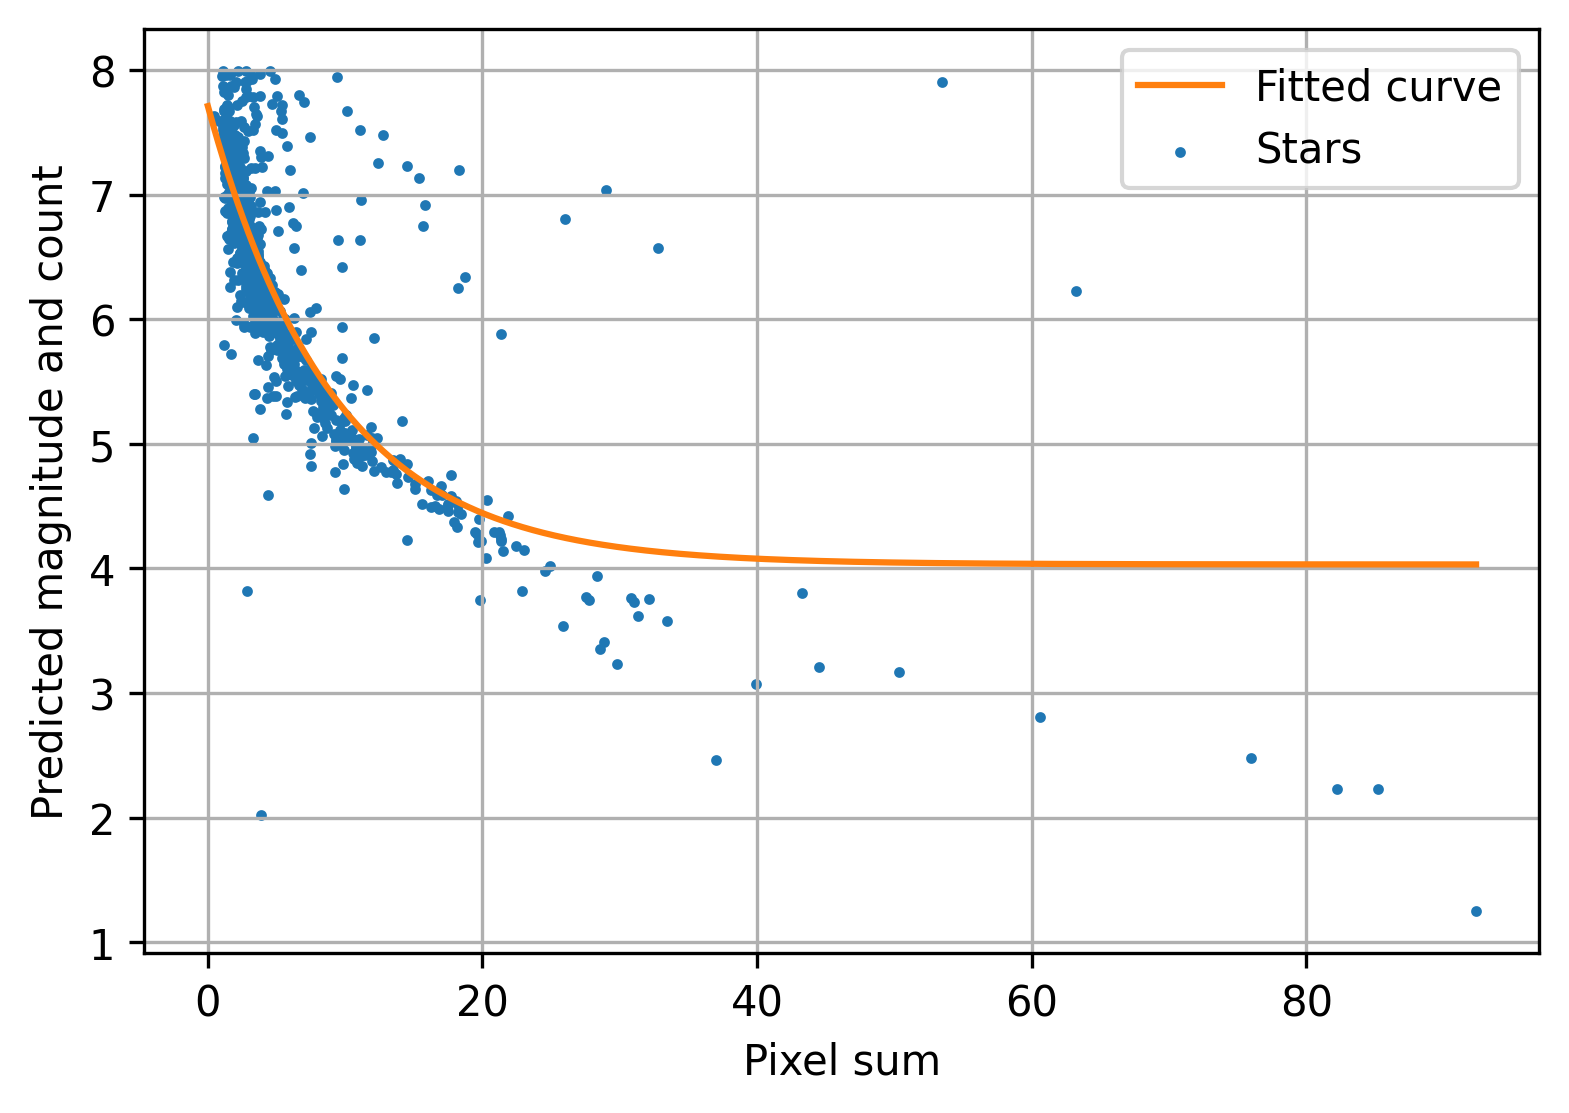
\includegraphics[width=\linewidth]{histogram_fitted.png}
    \caption{Fitted exponential function $f(x)$}
    \label{fig:fitted-exponential}
  \end{subfigure}
  \caption{}
\end{figure}

The magnitude of a star is a measure of the intensity of light it emits on a reverse
logarithmic scale. We want to predict the magnitude of the stars in the image for further
analysis. The pixel mask that was created in \autoref{sec:star-identification} gives us a
set of pixels with values in $[0, 1]$ for each star. This serves as the basis for the
estimation and will be summed up to get the total intensity of the star. As the
\texttt{floodFill} method selects pixels based only on the intensity difference to their
direct neighbors, the selection of pixels with a medium value is inconsistent.

\begin{figure}[tb]
  \centering
  \begin{subfigure}{.49\textwidth}
    \centering
    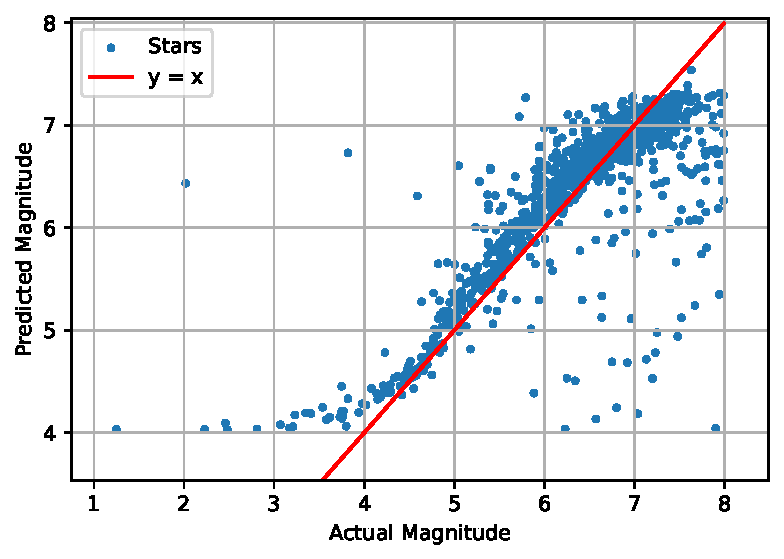
\includegraphics[width=\linewidth]{magnitude_prediction.pdf}
    \caption{Prediction with the exponential function $f(x)$}
    \label{fig:prediction-exponential}
  \end{subfigure}%
  \hfill
  \begin{subfigure}{.49\textwidth}
    \centering
    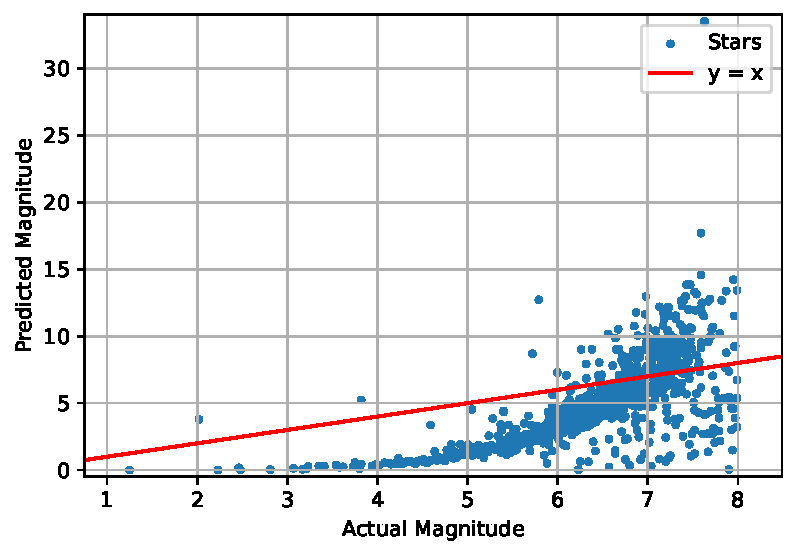
\includegraphics[width=\linewidth]{magnitude_prediction_log.pdf}
    \caption{Prediction with the logarithmic function $g(x)$}
    \label{fig:prediction-logarithmic}
  \end{subfigure}
  \caption{Comparison of the predicted magnitudes to the true magnitudes.}
  \label{fig:prediction}
\end{figure}

To get a more accurate selection, I first scaled the image using the function $s(x) =
  x^{0.1}$ (see \autoref{fig:kmeans-scaling}). This spreads out the values of the dimmer
pixels to make them more distinguishable. Then, I applied k-means clustering with $k =
  2$ to the pixels within the bounding box of each star. Pixels belonging to the cluster
with the higher mean are considered star-pixels, and background-pixels otherwise. The
clustering separates bright from dark pixels more consistently without any predefined
factor or shape. I chose centroid-based clustering, because it can guarantee two
clusters. For the implementation, I used the \texttt{KMeans} class from the
\texttt{scikit-learn} library \cite{scikit-learn}.

After refining the mask, I fitted an exponential function to the data. It takes the sum of
pixels, that were classified as star-pixels, as input and returns the magnitude. The
function is defined as
\begin{align*}
  f(x) = a \cdot \exp{\left(-b \left(\frac{x}{30} - c\right)\right)} + d,
\end{align*}
where $a$, $b$, $c$ and $d$ are the parameters to be fitted. The factor $30$ is used to
ensure convergence of the optimization algorithm. The parameters are fitted using the
\texttt{curve\_fit} method from the \texttt{scipy} library \cite{scipy2020}. The optimal
values of the parameters are $a = 0.47$, $b = 3.28$, $c = 0.63$ and $d = 4.03$ and the
resulting function is shown in \autoref{fig:fitted-exponential}.

I tested other functions, like a polynomial, hyperbolic, logarithmic and variations of
trigonometric functions. The function $g(x) = a \cdot \log(1 / x + b)$ would be the most
appropriate in the physical sense, as it is a convex function with $\lim_{0 \leftarrow x}
  g(x) = \infty$ which can produce negative values. However, having many points with a low
pixel sum meant that the fitted function assigned the same magnitude to all brighter
stars. A comparison of the magnitude predicted by the logarithmic function to the true
magnitudes is shown in \autoref{fig:prediction-logarithmic}. I settled on the exponential
function (\autoref{fig:fitted-exponential}) mentioned above, because it produced the
lowest mean squared error. For a pixel sum of 0, the function returns a magnitude of
$7.5$, which is the maximum magnitude of the stars in the image. Any star with a higher
magnitude is not distinguishable from noise. The function stagnates towards a magnitude of
$4$ from a pixel sum of $50$ onwards. This is likely due to a lack of training data and
saturation of the sensor for a majority of the pixels.

The mean squared error of the fit without the clustering step was $0.366$. With the
clustering, but without the scaling by $s(x)$, the error was $0.349$. The final error
after applying both mask refinement steps was $0.334$, which is a reduction of $9.6\%$
compared to the initial error. The MSE of the logarithmic function $g(x)$ was $0.452$. A
comparison of the predicted magnitudes to the true magnitudes is shown in
\autoref{fig:prediction}. The true magnitudes are on the x-axis and the predicted
magnitudes on the y-axis, with the red line $y = x$ for reference. The function is not
perfect, but it is a good approximation for the majority of stars. The outliers could be
due to the stars being matched to the wrong catalog star or two stars being recognized as
one object. Also, very bright stars are not estimated well, likely because they are
saturated in the image.

\subsection{Source-Count Distribution}
\label{sec:source-count-distribution}

A source-count distribution is a cumulative distribution of the number of sources ($N$)
brighter than a given flux density ($S$). It corresponds to the volume integration of
those stars which generate a received radiation flux of $S > S_0$ for a given flux density
$S_0$. Using the distance-luminosity relation $L(S) = 4 \pi r^2 S$, where $r$ is the
distance to the source, and integrating over the luminosity function $\Phi(L)$, we can
derive the general form of the source-count distribution as
\begin{align*}
  N(> S) = N_0 \cdot \left(\frac{S}{S_0}\right)^{-\frac{3}{2}},
\end{align*}
where $N_0$ and $S_0$ are normalization constants. The slope of the distribution is
determined by the power-law index -3/2. With the definition of the magnitude $m - m_0 =
  -2.5 \log_{10}{(S/S_0)}$, we can express the source-count distribution in terms of the
magnitude as
\begin{equation}
  \log_{10}{(N(< m))} = \log_{10}{(N_0)} + 0.6 \cdot (m - m_0).
  \label{eq:source-count}
\end{equation}
We can use this relation to verify the accuracy of the magnitude estimation. The
distribution of the magnitudes of the stars in the calibrated image, estimated by the
approach in \autoref{sec:magnitude-estimation}, is shown in
\autoref{fig:distribution-predicted}. For comparison, the same plot is shown for the stars
obtained from the SIMBAD database using the query in \autoref{lst:simbad-query} in
\autoref{fig:distribution-true}. I fitted the function in \autoref{eq:source-count} to the
cumulative distribution, with the slope, $N_0$ and $m_0$ as free parameters. From the fit,
I obtained a slope of $0.41$ for the predicted magnitudes and $0.51$ for the true
magnitudes, which is close to the expected value of $0.6$. One of the main reasons for the
deviation is likely the low accuracy of the predictor for bright stars. As no star
receives a magnitude of less than $4$, the distribution is inflated at the bright end,
which contributes to the lower slope. Also, the distribution would likely approach a slope
of $0.6$ more closely, if the distribution would include stars with a magnitude higher
than 8.0. I suspect this is the reason for the lower slope of the true magnitudes as well.

\begin{figure}[tb]
  \centering
  \begin{subfigure}{.49\textwidth}
    \centering
    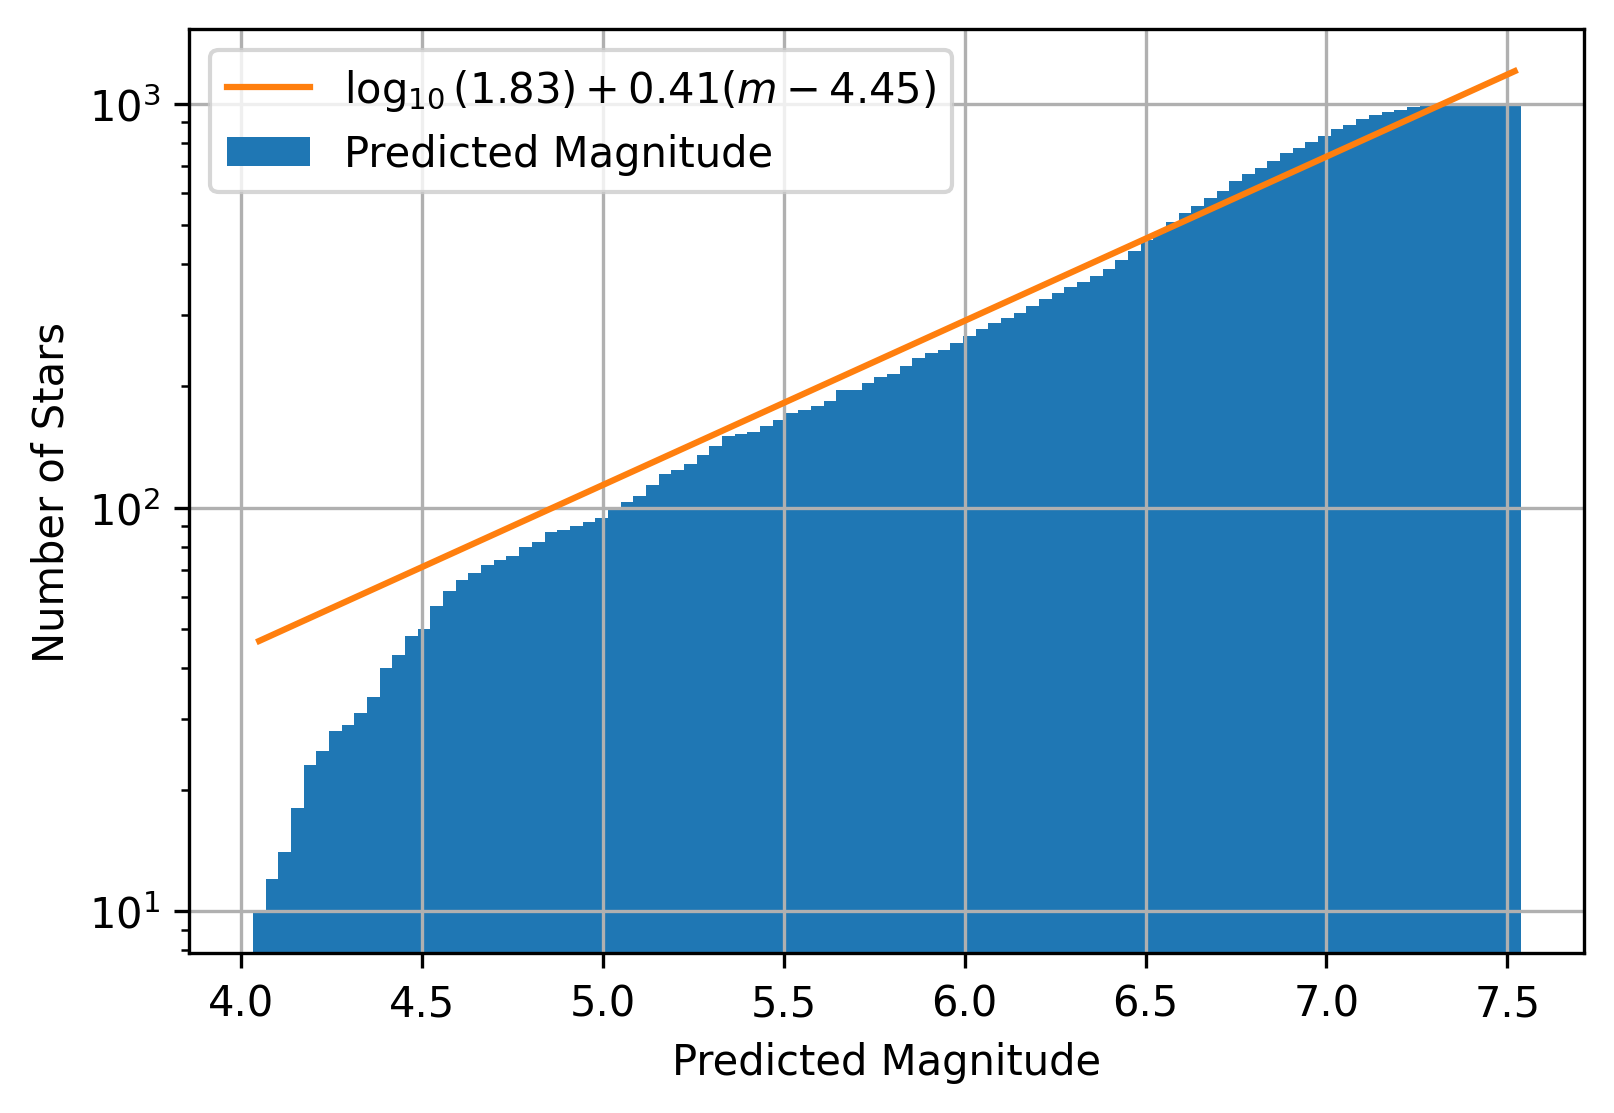
\includegraphics[width=\linewidth]{source_count_predicted.png}
    \caption{Prediction with the exponential function $f(x)$}
    \label{fig:distribution-predicted}
  \end{subfigure}%
  \hfill
  \begin{subfigure}{.49\textwidth}
    \centering
    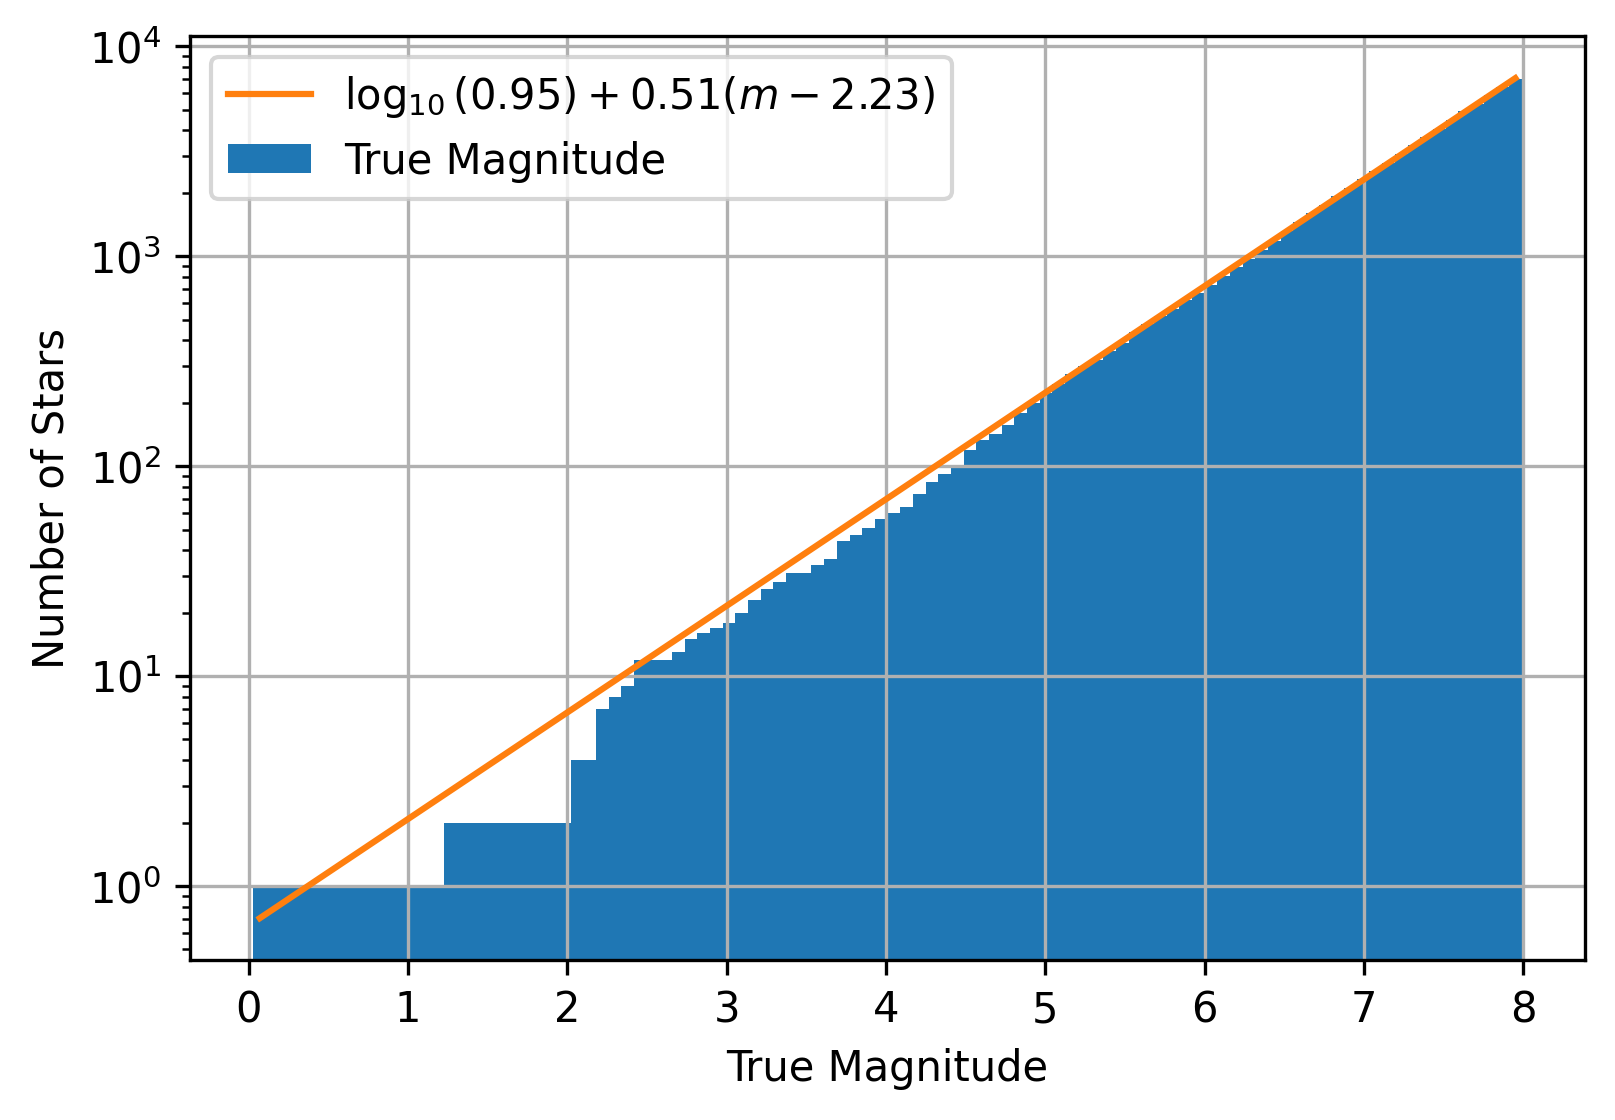
\includegraphics[width=\linewidth]{source_count_true.png}
    \caption{Prediction with the logarithmic function $g(x)$}
    \label{fig:distribution-true}
  \end{subfigure}
  \caption{}
  \label{fig:source-count}
\end{figure}


\section{Discussion}
\label{sec:discussion}

The goal of this project was to develop a program for the analysis of night sky images
and use it to estimate the source-count distribution of stars. The program consists of
the calibration of the input image, the identification of stars, matching them to a
catalog and estimating their magnitudes.

Judging by the results, the calibration of the image was successful. The faulty pixels
were corrected, the vignetting effect was removed, and the skyglow was reduced. I think
the biggest improvement would be to verify that the calibration works reliably under
different conditions. How accurate is the method for different cameras, lenses, ISO
settings and exposure times? How well does the method handle diffraction spike patterns?
What if objects obstruct the view or the image is taken in the presence of the moon? I was
not able to test these questions, but I am confident that my approach performs well for
wide-field images with no obstructing objects.

The identification of stars was also successful. The method was able to find the majority
of the stars that are visible in the image. The main problem was the distinction between
stars and noise. I manually found stars that were not recognized, but they were faint and
hard to distinguish from the background. Also, if the image is very blurry or out of
focus, the algorithm might not work well. It would be interesting to combine the flood
fill method with the template matching approach for small objects. This could help to
identify stars that are too faint for the current method. The subsequent steps were very
reliant on the accuracy of solving for the camera orientation. It would be possible to
improve the robustness of the solver by taking the brightness of the stars into account.
Also, the solver could be combined with the catalog matching step to make the intermediate
step unnecessary. When estimating the brightness using the pixel sum, a big reason for
inaccuracy was that the sensor was saturated for many of the bright stars. This introduced
a different slope in the data, which the exponential function could not capture. It could
be modeled by a more complex function, but it would need to avoid overfitting the dimmer
stars. The magnitude estimation does not work for stars with a magnitude lower than 4.0 or
higher than 8.0, due to the lack of training data. The source-count distribution was
estimated by fitting a power-law to the cumulative distribution of the magnitudes. The
slope of the distribution was close to the expected value of $0.6$, but the distribution
was inflated at the bright end. I suspect this was due to the low accuracy of the
predictor. However, the shape of the distribution does fit the expected form.

In conclusion, the program is a good starting point for the analysis of night sky images.
It is able to calibrate images and give a solid estimate of how bright the stars are. The
code is modular and can be used as a library or as a basis for further development.


\makebibliography

\newpage
\appendix

\section{Appendix}
\label{sec:appendix}

\subsection{ADQL Query for the SIMBAD Database}
\label{sec:simbad-query}

% Full resolution input image

% Matched stars labeled on image

\begin{lstlisting}[language=SQL, caption={
  ADQL query for the SIMBAD database to find stars in the field of view of the input image.
  "Star.." stands for "star or any sub category of star". The query can be executed at
  \url{https://simbad.cds.unistra.fr/simbad/sim-tap/}.
}, label={lst:simbad-query}]
SELECT COUNT(*)
FROM basic JOIN flux ON oidref = oid
WHERE otype = 'Star..'
      AND filter = 'V'
      AND flux < 8.0
      AND CONTAINS(POINT('ICRS', RA, DEC), BOX('ICRS', 312.708, 60.171, 64, 45)) = 1;
\end{lstlisting}

\newpage

\subsection{Histograms of Predicted Magnitudes}

\begin{figure}[htbp]
  \centering
  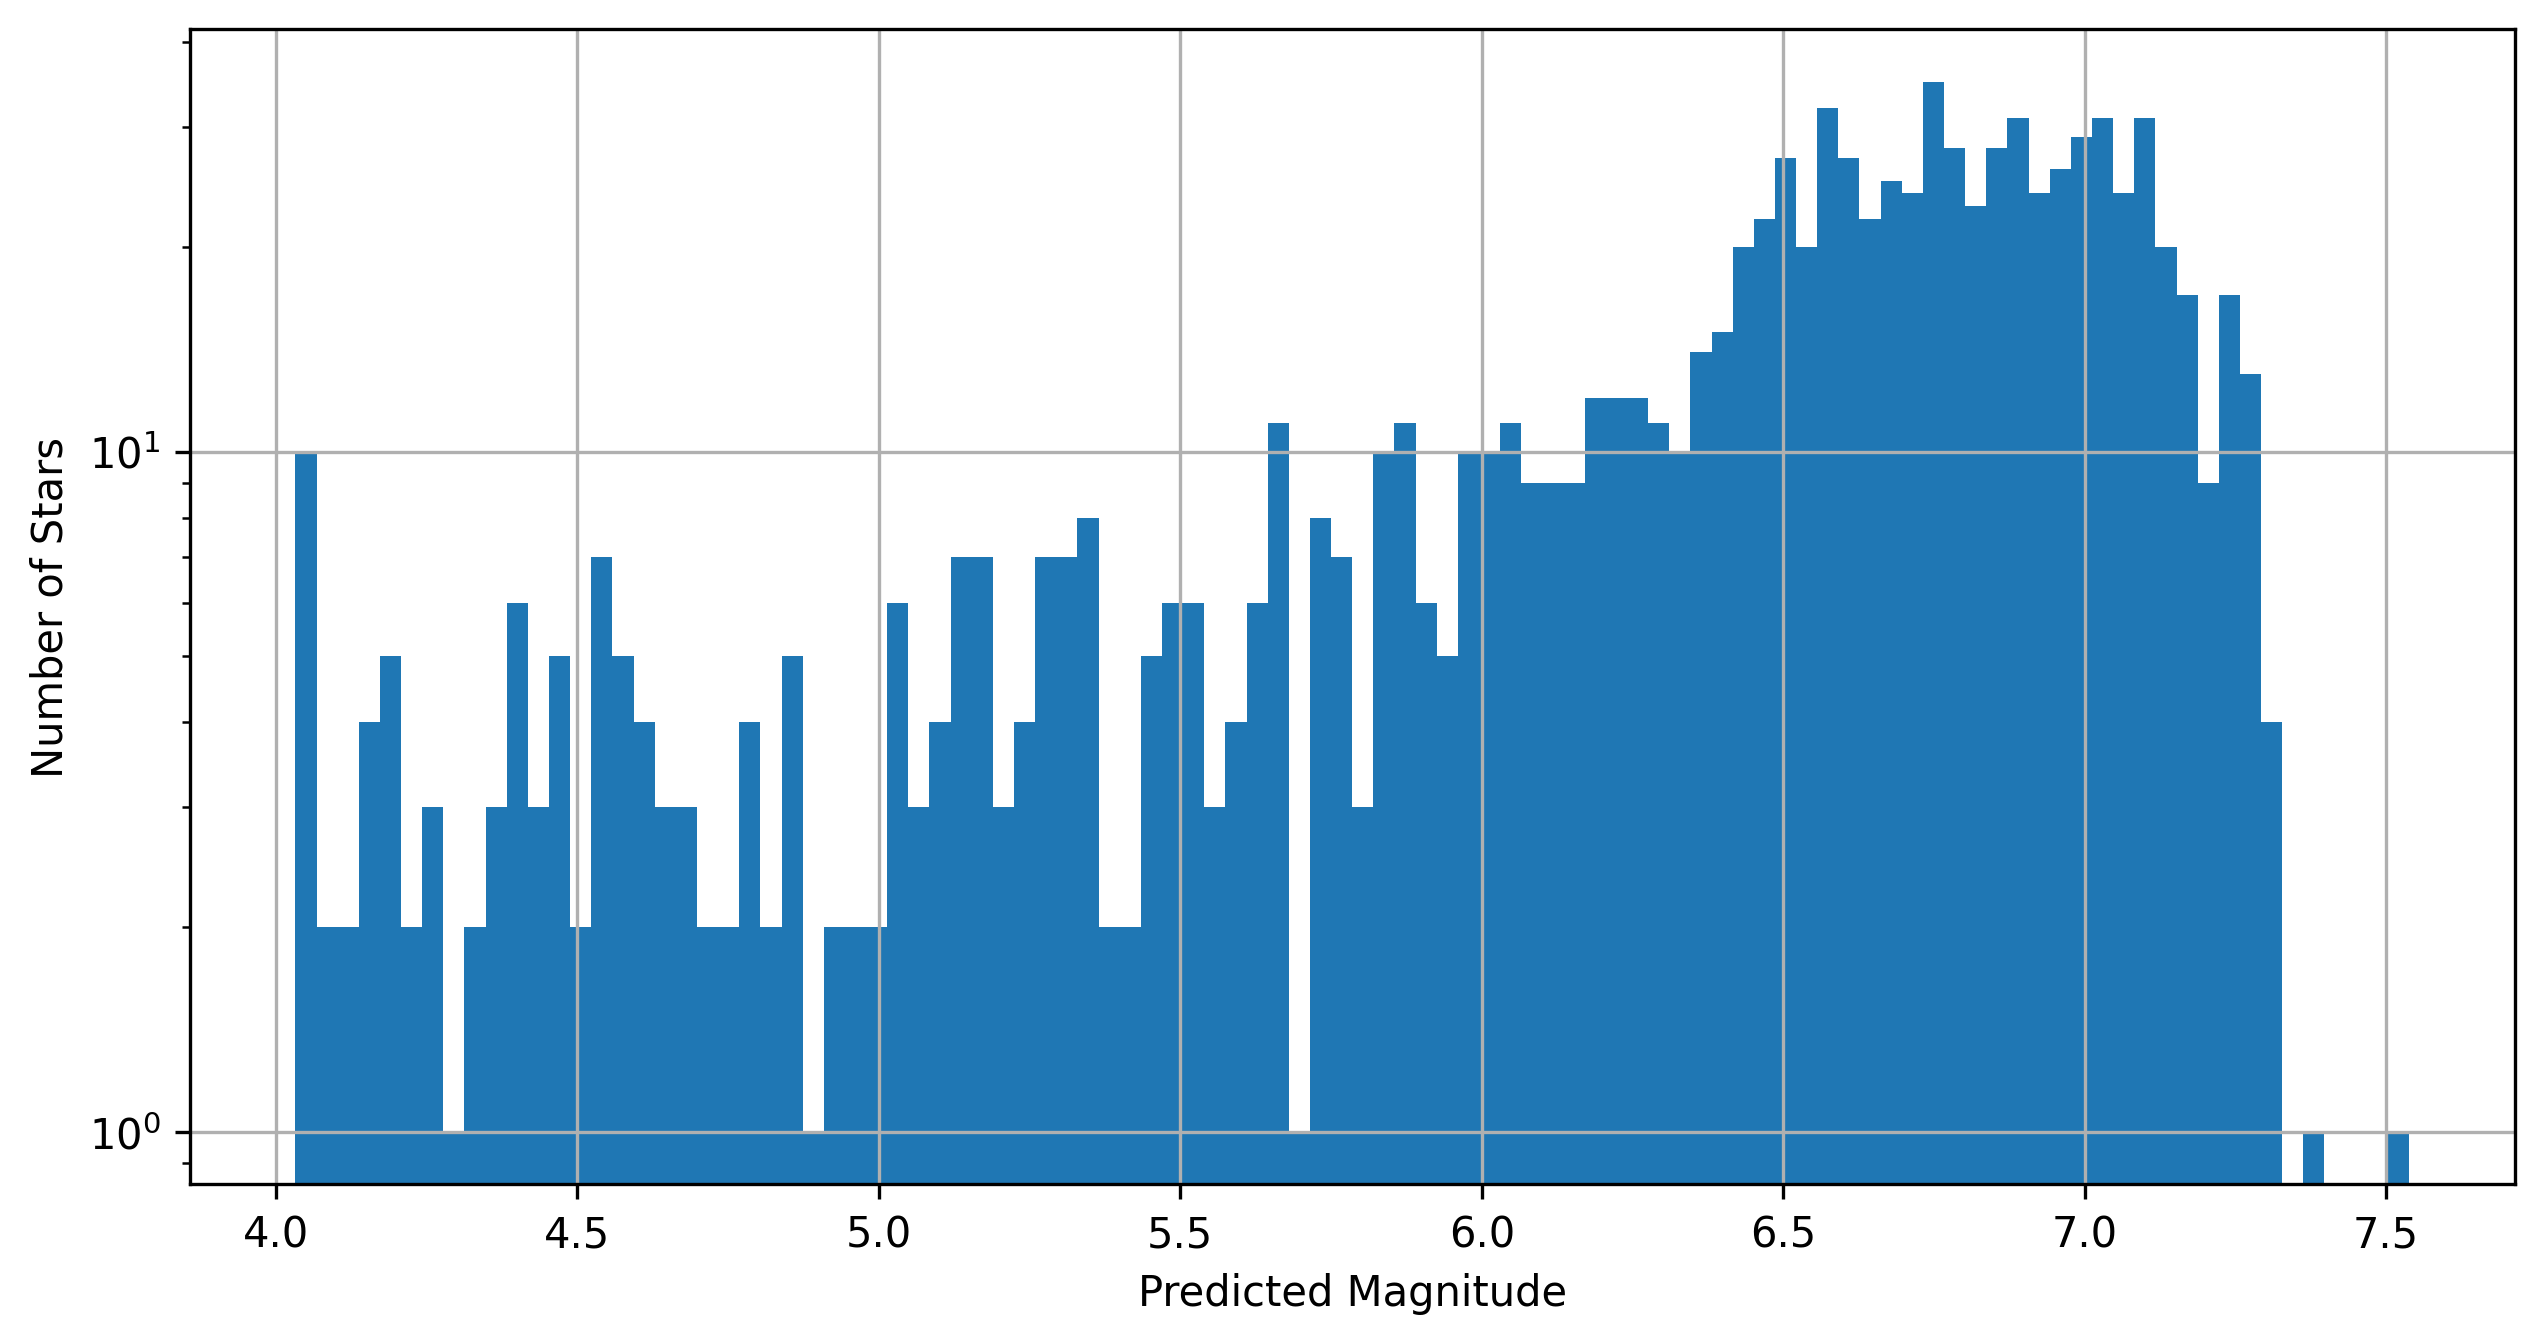
\includegraphics[width=.8\linewidth]{histogram_predicted_magnitudes.png}
  \caption{Histogram of the predicted magnitudes of stars in the input image.}
  \label{fig:hist-predicted-magnitudes}
\end{figure}

\begin{figure}[htbp]
  \centering
  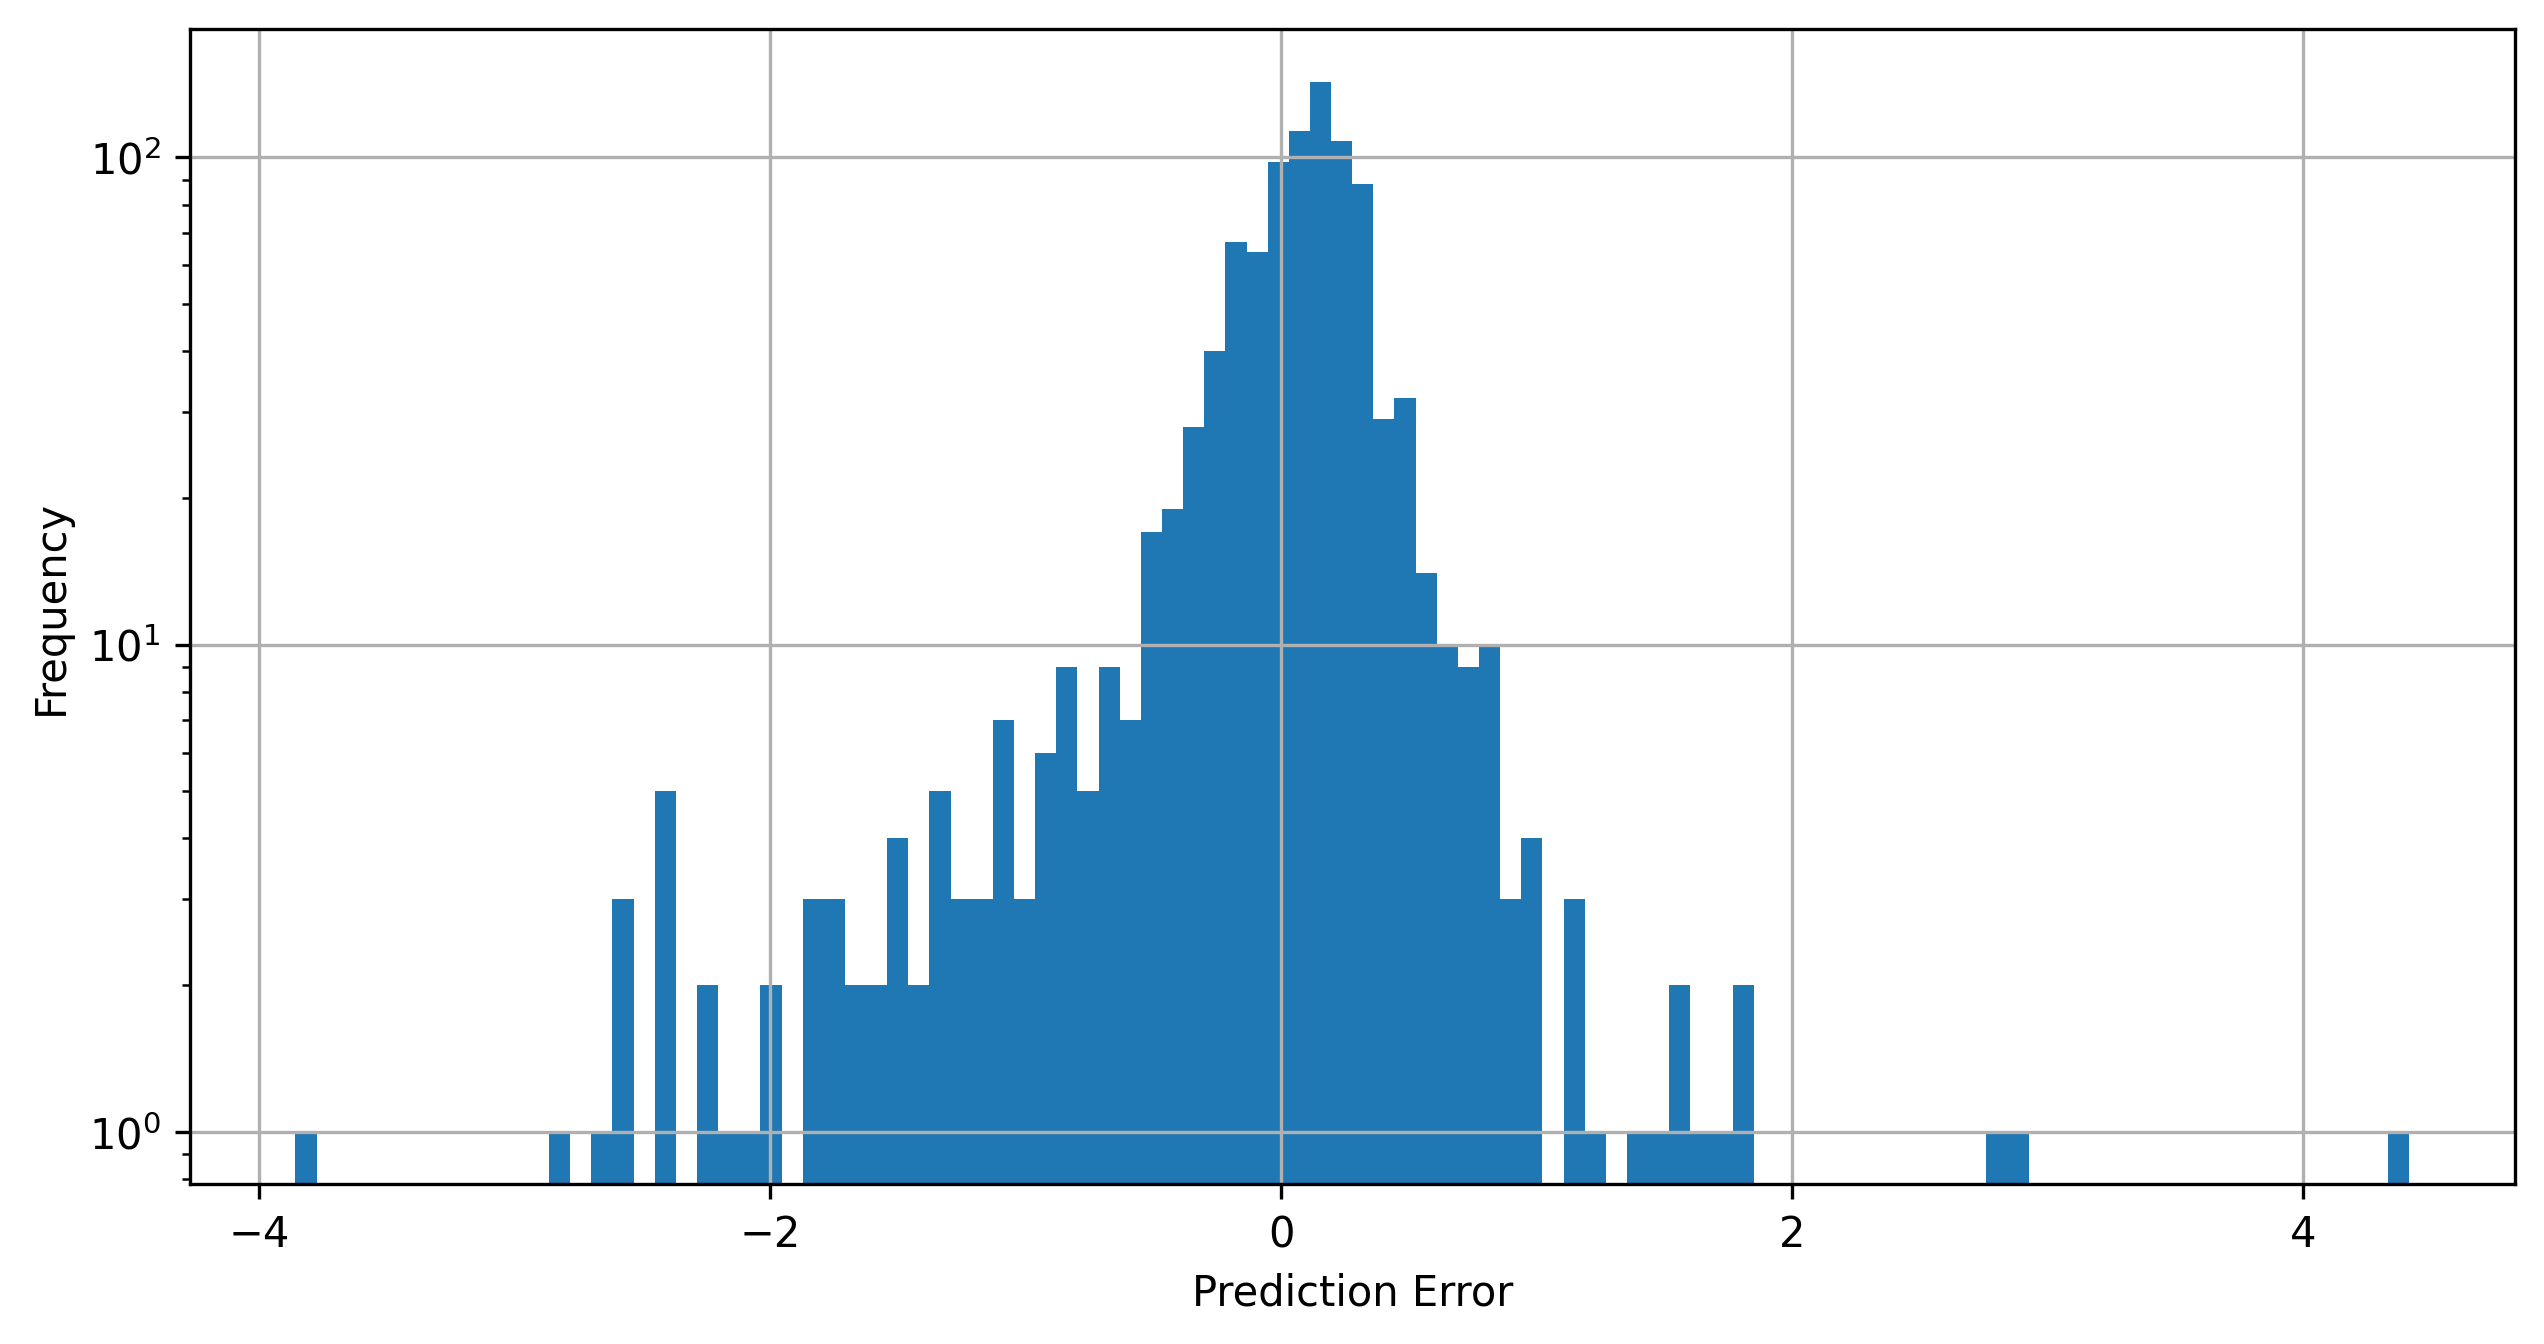
\includegraphics[width=.8\linewidth]{histogram_prediction_error.png}
  \caption{Histogram of the prediction error of the magnitudes of stars in the input image.}
  \label{fig:hist-predicted-error}
\end{figure}

\newpage

\subsection{Output of the Astrometry.net Service}

\begin{figure}[htbp]
  \centering
  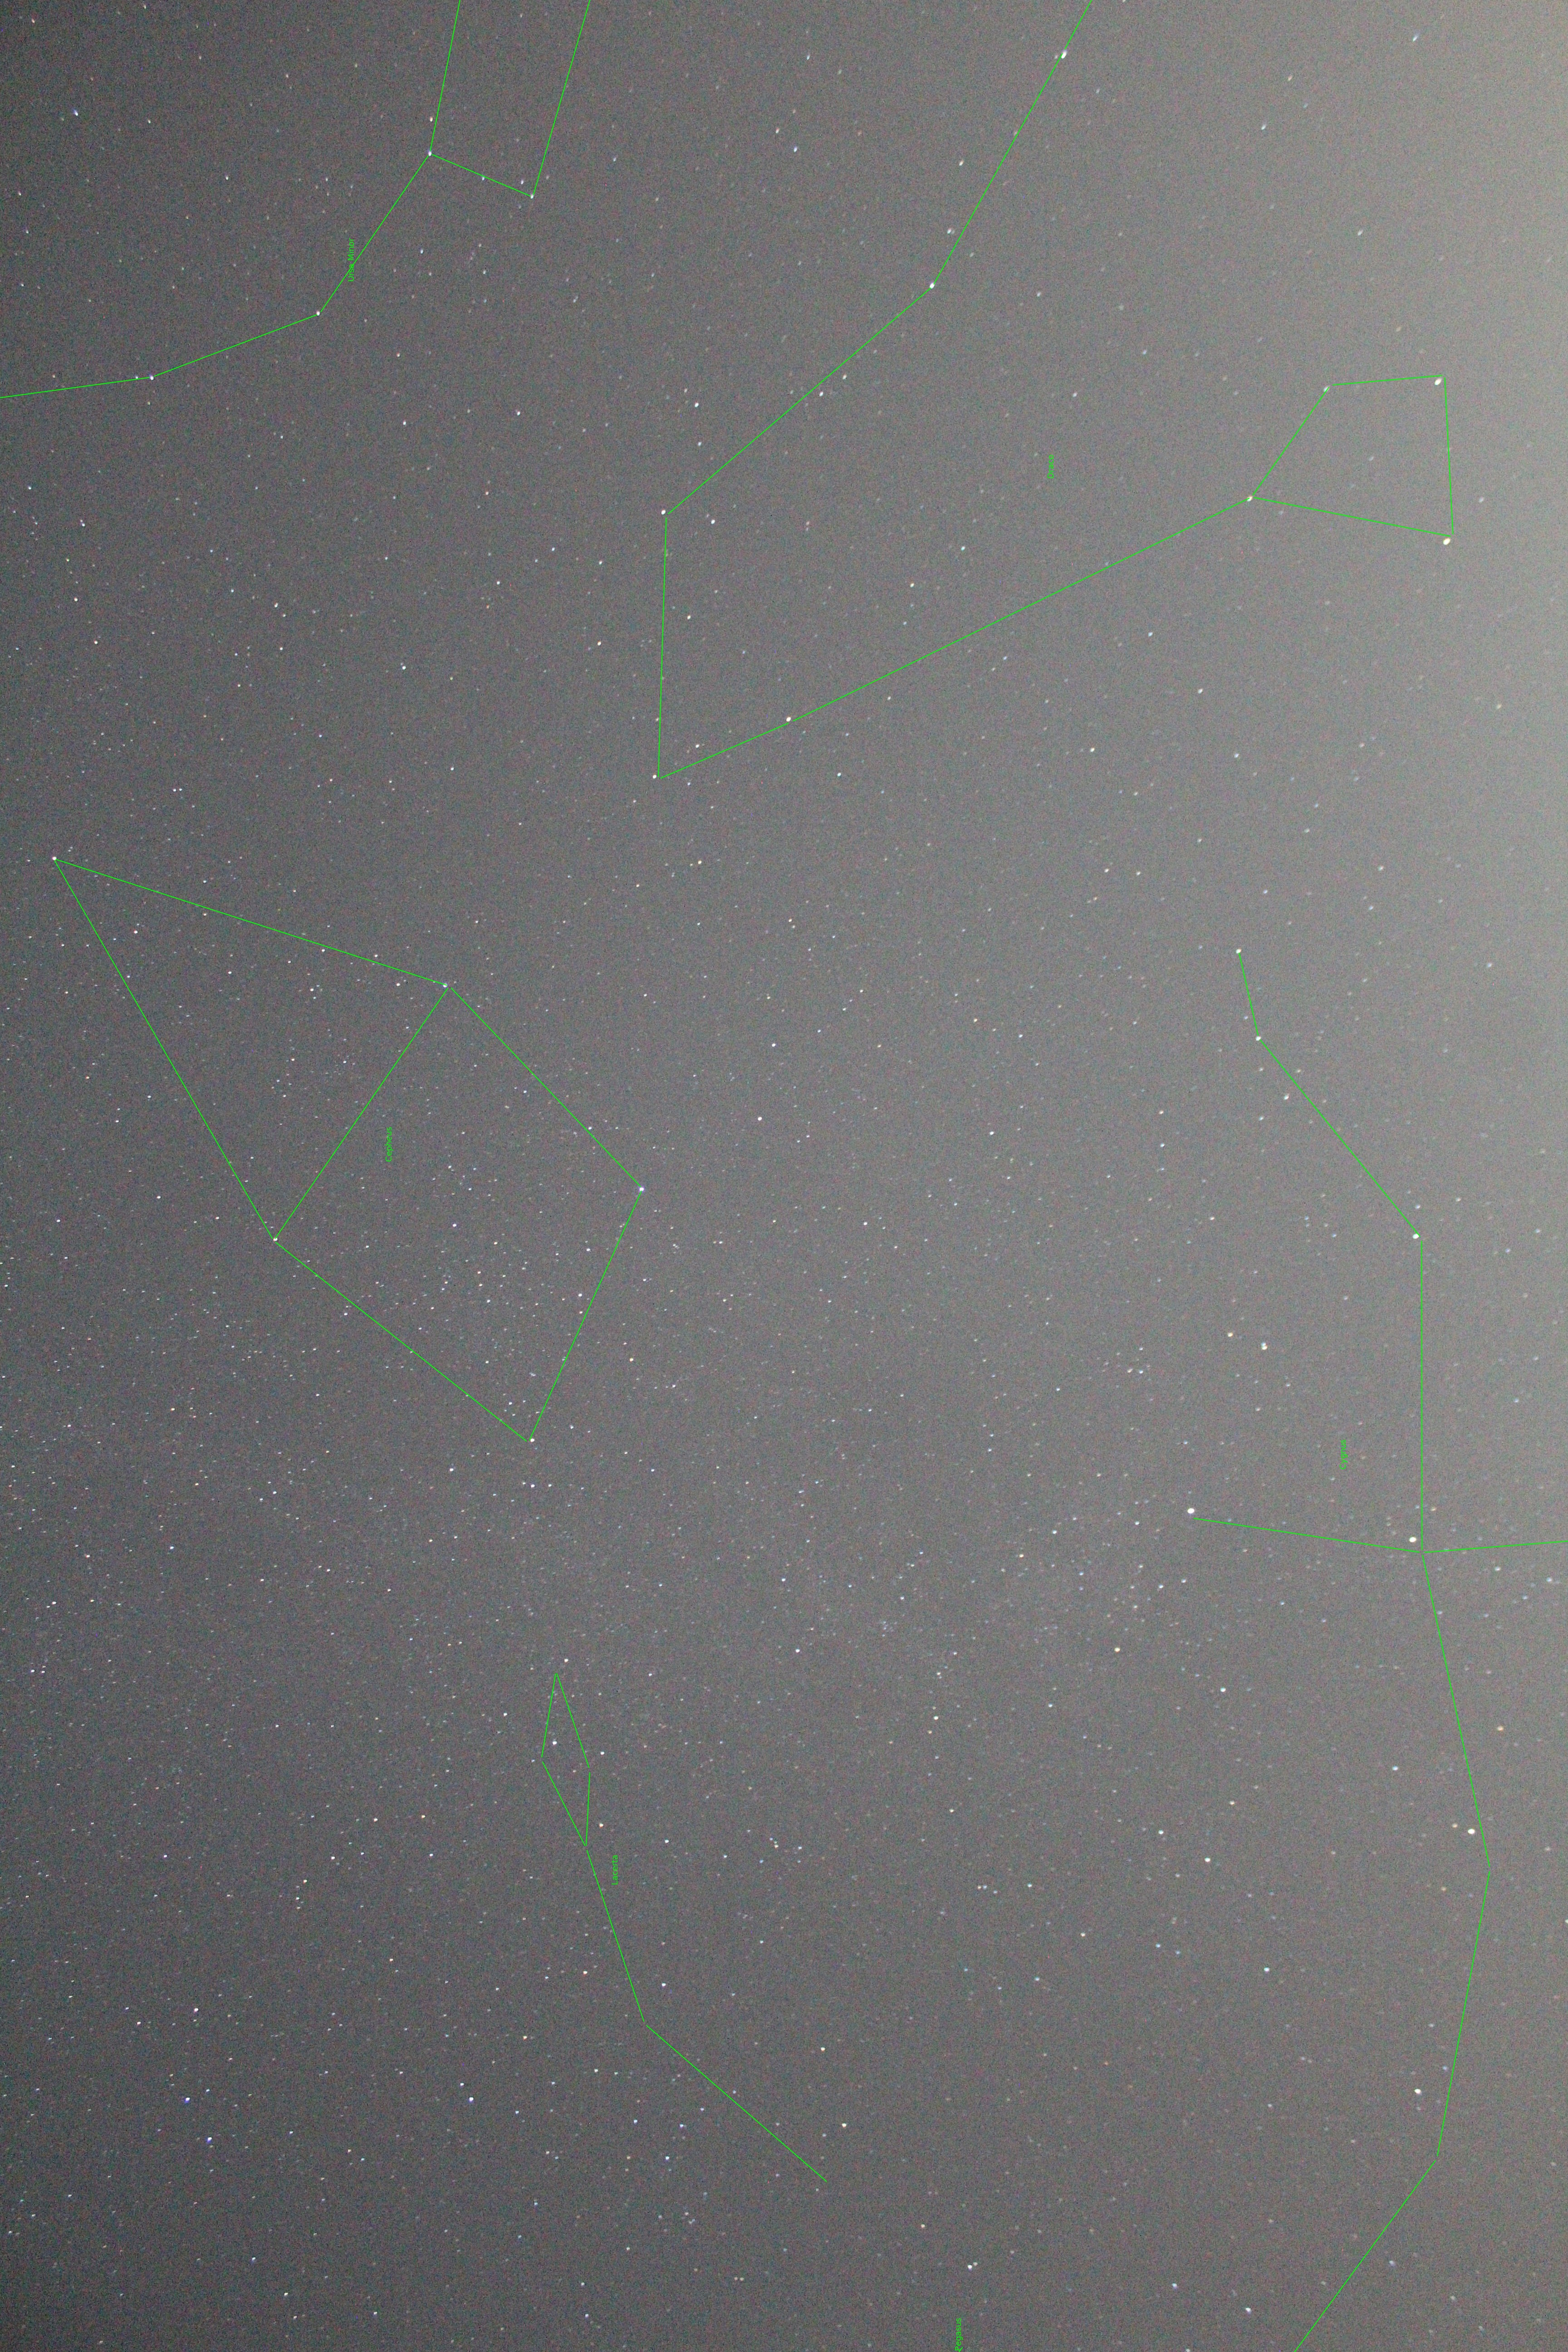
\includegraphics[width=.6\linewidth]{annotated.jpeg}
  \caption{Output of the Astrometry.net service for the input image. Find the results\\
    online at \url{https://nova.astrometry.net/user\_images/11597239\#annotated}.}
  \label{fig:astrometry-output}
\end{figure}

\end{document}

